%************************************************
\chapter{Randomised Strategies in the $\lambda$-calculus}
%************************************************
In the previous Chapter we have defined all the mathematical machinery needed for defining randomised strategies for ARSs, in the abstract. In this Chapter we focus on the $\lambda$-calculus, as defined in Chapter \ref{ch:lambda}, the target of our investigation. In deterministic strategies, the redex being reduced is typically chosen according to its position in the term. In randomised strategies we have more degrees of freedom. Intuitively we have to assign a probability to each redex of any term, making the sum to one. The space of possible choices is indeed very large. A first design choice could be the answer to the following question: should \emph{every} redex in a term being reduced with strictly positive probability? If the answer is yes, then one should decide how to give such probabilities. 
\section{The Uniform Strategy}
Maybe the most trivial way in which one could assign probabilities to redexes is in a \emph{uniform} way. Actually this was the first randomised strategy thought by Prof. Prakash Panangaden, who is ispired our work, through some conversations with Prof. Dal Lago. More formally, $\psuni$ is a randomised reduction strategy for the ARS $(\Lambda,\redbeta)$ such that for each reducible term $\termone$, ${\psuni=\mu\in\dist{\Lambda}}$. For each $\termtwo\in\Lambda$:
$$
\mu(\termtwo)=\begin{cases}
\frac{1}{|\rdxs{\termone}|} & \text{if }\termone\redbeta\termtwo ,\\
0 & \text{otherwise}.\\
\end{cases}
$$
where $\rdxs{\termone}$ is the set of rexes of $\termone$ and $|\rdxs{\termone}|$ its cardinality.
\begin{example}
	Let us consider a term $\termone = (\lambda x.\rdxone)\rdxtwo$
	where $\rdxone$ and $\rdxtwo$ are innermost redexes,
	$\rdxone\redbeta\rdxone'$ and
	$\rdxtwo\redbeta\rdxtwo'$. The stochastic process of reduction under strategy $\psuni$ can be represented by the tree in Figure \ref{figure:unitree}. Nodes are terms and two nodes are connected by an edge if and only if there is a strictly positive probability (written in the label) of reducing the father node into the child node.
\end{example}
\begin{figure}
	\begin{center}
		\fbox{
			\begin{minipage}{.96\textwidth}
				\begin{tikzpicture}[grow=down]
				\node[term] {$(\lambda x.\rdxone)\rdxtwo$}
				child {
					node[term] {$\rdxone\{\rdxtwo/x\}$}        
					edge from parent 
					node[below]  {$\frac{1}{3}$}
				}
				child {
					node[term] {$(\lambda x.\rdxone')\rdxtwo$}        
					edge from parent         
					node[left]  {$\frac{1}{3}$}
				}
				child {
					node[term] {$(\lambda x.\rdxone)\rdxtwo'$}        
					edge from parent         
					node[below]  {$\frac{1}{3}$}
				};
				\end{tikzpicture}
			\end{minipage}}
		\end{center}
	\caption{The tree (truncated after one step) representing the reduction of term $\termone = (\lambda x.\rdxone)\rdxtwo$ under randomised strategy $\psuni$.}
	\label{figure:unitree}
\end{figure}
Although very easy to define, the uniform strategy is not easy at all to study. In fact the number of redexes of terms along a reduction sequence can behave in a very complicated way. As we have seen in the previous Chapter, we study randomised strategies as FPARSs. In the case of the $\lambda$-calculus, the FPARS will be always in the form $(\Lambda_\mathsf{WN},\cdot)$. In fact it does not make any sense to consider terms which do not have normal form. Whether $(\Lambda_\mathsf{WN},\psuni)$ is AST is still an open problem, but for sure $(\Lambda_\mathsf{WN},\psuni)$ is not PAST, as we are going to prove showing a counterexample. 
\begin{example}
	Let us  consider the combinator $\termone=(\lambda x.\lambda y.y)\bm{\Delta_4}$, where $\bm{\Delta_4}=\bm{\Delta_2\Delta_2}$ and $\bm{\Delta_2}= \lambda x.(xx)(xx)$. We observe that $\bm{\Delta_4}$ reduces to $\bm{\Delta_4\Delta_4}$. Thus, if we do not reduce leftmost, the number of redexes grows linearly with the length of the reduction sequence. Instead, reducing leftmost, we reach the normal form immediately. Considering the computation $|(\rho_i)|_{i\in\mathbb{N}}$ starting from $\rho_0=\textbf{Dirac}(\termone)$ (in Figure \ref{figure:delta2}) we can compute the sequence $|\rho_i|$.
	\begin{equation*}
	\begin{split}
	|\rho_0|&=1\,,\\
	|\rho_1|&=1\,,\\
	|\rho_2|&=|\rho_1|-|\rho_1|\frac{1}{2}\,,\\
	|\rho_3|&=|\rho_2|-|\rho_2|\frac{1}{3}\,,\\
	|\rho_i|&=|\rho_{i-1}|-|\rho_{i-1}|\frac{1}{i}=|\rho_{i-1}|\left( 1-\frac{1}{i}\right).
	\end{split}
	\end{equation*}
	The recurrence relation in the last line can be solved analytically and yields $|\rho_i|=\frac{1}{i}$ for each $i\geq 1$. Thus $(\Lambda_\mathsf{WN},\psuni)$ is not PAST since 
	$$
	\nsteps{\psuni}(\termone)=\sum\limits_{i=1}^{\infty} \left|\rho_i\right|=\sum\limits_{i=1}^{\infty} \frac{1}{i}=+\infty.
	$$
\end{example}
\begin{figure}
	\begin{center}
		\fbox{
			\begin{minipage}{.96\textwidth}
				\begin{tikzpicture}[grow=down]
				\node[term] {$(\lambda x.\lambda y.y)\bm{\Delta_4}$}
				child {
					node[term] {$\lambda y.y$}        
					edge from parent         
					node[above]  {$\frac{1}{2}$}
				}
				child {
					node[term] {$(\lambda x.\lambda y.y)(\bm{\Delta_4\Delta_4})$}        
					child {
						node[term] {$\lambda y.y$}        
						edge from parent         
						node[above]  {$\frac{1}{3}$}
					}
					child {
						node[term] {$(\lambda x.\lambda y.y)((\bm{\Delta_4}\bm{\Delta_4})\bm{\Delta_4})$}
						edge from parent         
						node[right]  {$\frac{1}{3}$}
					}
					child {
						node[term] {$(\lambda x.\lambda y.y)(\bm{\Delta_4}(\bm{\Delta_4\Delta_4}))$}
						edge from parent         
						node[above]  {$\frac{1}{3}$}
					}
					edge from parent         
					node[above]  {$\frac{1}{2}$}
				};
				\end{tikzpicture}
			\end{minipage}}
		\end{center}
		\caption{The tree (truncated after two steps) representing the reduction of term $\termone = (\lambda x.\lambda y.y)\bm{\Delta_4}$ under randomised strategy $\psuni$.}
		\label{figure:delta2}
	\end{figure}
\section{The Strategy $P_\varepsilon$}
In real programming languages we would like to have a normalising strategy, or at least, since we are in probabilistic context, a positive almost-surely normalising one. For this reason we devised a new strategy for the $\lambda$-calculus $(\Lambda,\redbeta)$, more simple and traditional, since it mixes leftmost-outermost and rightmost-innermost strategies. If $\varepsilon\in[0,1]$, call $\mathsf{P}_\varepsilon$ the strategy in which the leftmost redex is reduced with probability $\varepsilon$ and the rightmost one with probability $1-\varepsilon$. Formally, given a reducible term $\termone$, $\mathsf{P}_\varepsilon(\termone)=\mu$ such that for each $\termtwo\in\Lambda$:
$$
\mu(\termtwo)=\begin{cases}
\varepsilon & \text{if }\termone\redbeta\termtwo\text{ and the }\pslo\text{-redex is reduced,}\\
1-\varepsilon & \text{if }\termone\redbeta\termtwo\text{ and the }\psri\text{-redex is reduced,}\\
0 & \text{otherwise}.\\
\end{cases}
$$
\begin{notation}
	For the FPARS $(\Lambda,\mathsf{P}_\varepsilon)$ and $\termone\in\Lambda$, we define the function $\explen{\termone}:[0,1]\rightarrow\mathbb{R}\cup\{+\infty\}$, where
	$\explen{\termone}(\varepsilon)=\nsteps{\mathsf{P}_\varepsilon}(\termone)$.
\end{notation}
\begin{example}
	Let us consider the term $\termone=(\lambda x.y)\bm{\Omega}$ where $\bm{\Omega}=\bm{\omega\omega}$  with $\bm{\omega}=\lambda x.xx$. There are two possible representations of the development of the strategy $\mathsf{P}_\varepsilon$ for this term, one as an infinite tree (Figure \ref{figure:trees}a) and another one as a cyclic graph (Figure \ref{figure:trees}b). According to the different representations, we can compute in different ways the probability of reaching normal form and the average derivation length.
	\begin{itemize}
		\item
		We start considering the strategy as an infinite tree. In this way the probability  $\mathsf{Pr}_{\mathsf{NF}}^{\termone}$ of reaching normal form from $\termone$ is obtained summing the probabilities $\mathsf{Pr}_n^{\termone}$ of reaching normal form from $\termone$ in $n$ steps. Since
		$$
		\mathsf{Pr}_n^{\termone}(\varepsilon)=\varepsilon(1-\varepsilon)^{n-1}\,,
		$$
		$$
		\mathsf{Pr}_{\mathsf{NF}}^{\termone}=\sum_{n=1}^{\infty}\mathsf{Pr}_n^{\termone}=\sum_{n=1}^{\infty}\varepsilon\left( 1-\varepsilon\right)^{n-1}=\varepsilon\frac{1}{1-(1-\varepsilon)}=1.
		$$
		The average derivation length is then
		$$
		\explen{\termone}(\varepsilon)=\sum_{n=1}^{\infty}n\mathsf{Pr}_n^{\termone}= \sum_{n=1}^{\infty}n\varepsilon(1-\varepsilon)^{n-1}=\frac{1}{\varepsilon}.
		$$
		\item
		Considering the strategy as a cyclic graph yields instead the following two equations:
		\begin{equation*}\begin{split}
				\mathsf{Pr}_{\mathsf{NF}}^{\termone} =& 1\cdot\varepsilon + (1-\varepsilon)\mathsf{Pr}_{\mathsf{NF}}^{\termone}\\
				\explen{\termone}(\varepsilon)=& 1\cdot\varepsilon + (1+\explen{\termone}(\varepsilon))(1-\varepsilon)
			\end{split}\end{equation*}
			which yield the same results as before.
		\end{itemize}
	%Moreover the reader can note the analogy with the abstract setting of Example \ref{example:pars}.
\end{example}
\begin{figure}
	\begin{center}
		\fbox{
			\begin{minipage}{.96\textwidth}
				\begin{center}
					\tikzstyle{level 1}=[level distance=1.8cm, sibling distance=2.5cm]
					\tikzstyle{level 2}=[level distance=1.8cm, sibling distance=2.5cm]
					\subfloat[]{{\begin{tikzpicture}[grow=down]
							
						\node[term] {$(\lambda x.y)\bm{\Omega}$}
						child {
							node[term] {$y$}        
							edge from parent         
							node[left]  {$\varepsilon$}
						}
						child {
							node[term] {$(\lambda x.y)\bm{\Omega}$}        
							child {
								node[term] {$y$}        
								edge from parent         
								node[left]  {$\varepsilon$}
							}
							child {
								node[term,label=below:{\begin{rotate}{-90}{$\cdots$}\end{rotate}}] {$(\lambda x.y)\bm{\Omega}$}
								edge from parent         
								node[right]  {$1-\varepsilon$}
							}
							edge from parent         
							node[right]  {$1-\varepsilon$}
						};
						\end{tikzpicture}}}
				\qquad\qquad\qquad
				\tikzstyle{level 1}=[level distance=3cm, sibling distance=2.5cm]
				\subfloat[]{{\begin{tikzpicture}[grow=down]
						\node[term]  (M) {$(\lambda x.y)\bm{\Omega}$}
						child {
							node[term] {$y$}        
							edge from parent         
							node[left]  {$\varepsilon$}
						};
						\path[-]
						(M) edge [loop above] node {$1-\varepsilon$} ();
						
						\end{tikzpicture}}}
			\end{center}
		\end{minipage}}
	\end{center}
	\caption{The tree (a) and the cyclic graph (b) representing the reduction sequence of $\termone$.}
	\label{figure:trees}
\end{figure}
The first Theorem we are going to prove around $\mathsf{P}_\varepsilon$ states that $\mathsf{P}_\varepsilon$ is an almost-surely normalising strategy. The key aspect of this proof is that the $\pslo$-redex has always the \emph{same} probability $\varepsilon$ of being reduced, along the whole reduction sequence.
\begin{theorem}
	The FPARS $(\Lambda_\mathsf{WN},\mathsf{P}_\varepsilon)$ is PAST whenever $\varepsilon>0$.
\end{theorem}
\begin{proof}
	We use Foster's Theorem to prove the claim. Thus we have to find a suitable Lyapunov function $V$.
	We consider $V=\nsteps{\pslo}$. Certainly condition (1) is verified since $\nsteps{\pslo}\left(\termone\right)\geq0$ for each $\termone\in\Lambda_\mathsf{WN}$. We have to verify (2). Suppose $\mathsf{P}_\varepsilon(\termone)=\mu$. If $\termone\redlo\termtwo$ and $\termone\redri\termthree$, by Lemma~\ref{lemma:derivationlength} we can write:
	\begin{equation*}
	\begin{split}
	\nsteps{\pslo}\left( \mu\right) & = \nsteps{\pslo}(\termtwo) \cdot \varepsilon+ \nsteps{\pslo}(\termthree)\cdot (1-\varepsilon)\\
	& \leq \left( \nsteps{\pslo}\left( \termone\right)-1\right)  \cdot \varepsilon + \nsteps{\pslo}(\termone)\cdot (1-\varepsilon)\\
	& = \varepsilon\cdot\nsteps{\pslo}\left( \termone\right)-\varepsilon + \nsteps{\pslo}\left( \termone\right)\cdot\left( 1-\varepsilon\right)\\
	& = \nsteps{\pslo}\left( \termone\right)-\varepsilon.
	\end{split}
	\end{equation*}
	Since $0\leq\varepsilon\leq 1$, $\nsteps{\pslo}\left(M\right)>_{\varepsilon}\nsteps{\pslo}\left(\mu\right)$ for each normalising term $\termone$.
	Then, if $\varepsilon>0$, $(\Lambda_\mathsf{WN},\mathsf{P}_\varepsilon)$ is PAST and the average number of steps to normal form of a term $\termone$ reduced with strategy $\mathsf{P}_\varepsilon$ is bounded by
	$\frac{\nsteps{\pslo}\left( \termone\right)}{\varepsilon}$.
\end{proof}
The bound we obtain on $\explen{\termone}(\varepsilon)$ from the above proof is very loose and thus it does not give us any information on the actual nature of the function $\explen{\termone}(\varepsilon)$. We show, by means of an example, that the strategy $\mathsf{P}_\varepsilon$ is non-trivial, i.e. there exists a term $\termone$ and $0<\varepsilon<1$, such that $\explen{\termone}(\varepsilon)<\explen{\termone}(1)=\nsteps{\pslo}(\termone)<\explen{\termone}(0)=\nsteps{\psri}(\termone)$.
\begin{example}
	Let us consider a family of terms $\termone_n=\termtwo\termthree_n$ where:
	$$
	\termtwo = \lambda x.\underbrace{((\lambda y.z)\bm{\Omega})}_\termfour x\qquad
	\termthree_n = C_n\underbrace{((\lambda x.x)y)}_\termfive\qquad
	C_n = \lambda  x.\underbrace{xx\cdots x}_{n\text{ times}}
	$$
	In Figure \ref{figure:probtree} the labeled graph representing all possible traces of the stochastic reduction process is sketched. After quite simple computations, i.e. taking the weighted mean of the legths of all possible paths from the root to the normal form, one can derive the following expression: 
	$$
	\explen{\termone_n}(\varepsilon)=(n-3)\varepsilon^3+4\varepsilon^2+\frac{2}{\varepsilon}.
	$$
	Clearly for $\varepsilon=0$ the expression diverges. If $n\geq 2$ there is a minimum for $0<\varepsilon<1$, and thus $\explen{\termone_n}(\varepsilon) <\explen{\termone_n}(1)=\nsteps{\pslo}(\termone_n) <\explen{\termone_n}(0)= \nsteps{\psri}(\termone_n)=+\infty$. $\explen{\termone_9}(\varepsilon)$ is plotted in Figure \ref{figure:plot}.
	\begin{figure}
		\fbox{
			\begin{minipage}{.96\textwidth}
				\centering
				\scalebox{1}{\begin{adjustbox}{clip,trim=2.5in 2in 0.5in 0.4in}%% Creator: Matplotlib, PGF backend
%%
%% To include the figure in your LaTeX document, write
%%   \input{<filename>.pgf}
%%
%% Make sure the required packages are loaded in your preamble
%%   \usepackage{pgf}
%%
%% Figures using additional raster images can only be included by \input if
%% they are in the same directory as the main LaTeX file. For loading figures
%% from other directories you can use the `import` package
%%   \usepackage{import}
%% and then include the figures with
%%   \import{<path to file>}{<filename>.pgf}
%%
%% Matplotlib used the following preamble
%%   \usepackage{fontspec}
%%   \setmainfont{DejaVu Serif}
%%   \setsansfont{DejaVu Sans}
%%   \setmonofont{DejaVu Sans Mono}
%%
\begingroup%
\makeatletter%
\begin{pgfpicture}%
\pgfpathrectangle{\pgfpointorigin}{\pgfqpoint{6.400000in}{4.800000in}}%
\pgfusepath{use as bounding box, clip}%
\begin{pgfscope}%
\pgfsetbuttcap%
\pgfsetmiterjoin%
\definecolor{currentfill}{rgb}{1.000000,1.000000,1.000000}%
\pgfsetfillcolor{currentfill}%
\pgfsetlinewidth{0.000000pt}%
\definecolor{currentstroke}{rgb}{1.000000,1.000000,1.000000}%
\pgfsetstrokecolor{currentstroke}%
\pgfsetdash{}{0pt}%
\pgfpathmoveto{\pgfqpoint{0.000000in}{0.000000in}}%
\pgfpathlineto{\pgfqpoint{6.400000in}{0.000000in}}%
\pgfpathlineto{\pgfqpoint{6.400000in}{4.800000in}}%
\pgfpathlineto{\pgfqpoint{0.000000in}{4.800000in}}%
\pgfpathclose%
\pgfusepath{fill}%
\end{pgfscope}%
\begin{pgfscope}%
\pgfsetbuttcap%
\pgfsetmiterjoin%
\definecolor{currentfill}{rgb}{1.000000,1.000000,1.000000}%
\pgfsetfillcolor{currentfill}%
\pgfsetlinewidth{0.000000pt}%
\definecolor{currentstroke}{rgb}{0.000000,0.000000,0.000000}%
\pgfsetstrokecolor{currentstroke}%
\pgfsetstrokeopacity{0.000000}%
\pgfsetdash{}{0pt}%
\pgfpathmoveto{\pgfqpoint{0.800000in}{0.528000in}}%
\pgfpathlineto{\pgfqpoint{5.760000in}{0.528000in}}%
\pgfpathlineto{\pgfqpoint{5.760000in}{4.224000in}}%
\pgfpathlineto{\pgfqpoint{0.800000in}{4.224000in}}%
\pgfpathclose%
\pgfusepath{fill}%
\end{pgfscope}%
\begin{pgfscope}%
\pgfsetbuttcap%
\pgfsetroundjoin%
\definecolor{currentfill}{rgb}{0.000000,0.000000,0.000000}%
\pgfsetfillcolor{currentfill}%
\pgfsetlinewidth{0.803000pt}%
\definecolor{currentstroke}{rgb}{0.000000,0.000000,0.000000}%
\pgfsetstrokecolor{currentstroke}%
\pgfsetdash{}{0pt}%
\pgfsys@defobject{currentmarker}{\pgfqpoint{0.000000in}{-0.048611in}}{\pgfqpoint{0.000000in}{0.000000in}}{%
\pgfpathmoveto{\pgfqpoint{0.000000in}{0.000000in}}%
\pgfpathlineto{\pgfqpoint{0.000000in}{-0.048611in}}%
\pgfusepath{stroke,fill}%
}%
\begin{pgfscope}%
\pgfsys@transformshift{0.800000in}{2.376000in}%
\pgfsys@useobject{currentmarker}{}%
\end{pgfscope}%
\end{pgfscope}%
\begin{pgfscope}%
\pgftext[x=0.800000in,y=2.278778in,,top]{\sffamily\fontsize{10.000000}{12.000000}\selectfont -1.00}%
\end{pgfscope}%
\begin{pgfscope}%
\pgfsetbuttcap%
\pgfsetroundjoin%
\definecolor{currentfill}{rgb}{0.000000,0.000000,0.000000}%
\pgfsetfillcolor{currentfill}%
\pgfsetlinewidth{0.803000pt}%
\definecolor{currentstroke}{rgb}{0.000000,0.000000,0.000000}%
\pgfsetstrokecolor{currentstroke}%
\pgfsetdash{}{0pt}%
\pgfsys@defobject{currentmarker}{\pgfqpoint{0.000000in}{-0.048611in}}{\pgfqpoint{0.000000in}{0.000000in}}{%
\pgfpathmoveto{\pgfqpoint{0.000000in}{0.000000in}}%
\pgfpathlineto{\pgfqpoint{0.000000in}{-0.048611in}}%
\pgfusepath{stroke,fill}%
}%
\begin{pgfscope}%
\pgfsys@transformshift{1.420000in}{2.376000in}%
\pgfsys@useobject{currentmarker}{}%
\end{pgfscope}%
\end{pgfscope}%
\begin{pgfscope}%
\pgftext[x=1.420000in,y=2.278778in,,top]{\sffamily\fontsize{10.000000}{12.000000}\selectfont -0.75}%
\end{pgfscope}%
\begin{pgfscope}%
\pgfsetbuttcap%
\pgfsetroundjoin%
\definecolor{currentfill}{rgb}{0.000000,0.000000,0.000000}%
\pgfsetfillcolor{currentfill}%
\pgfsetlinewidth{0.803000pt}%
\definecolor{currentstroke}{rgb}{0.000000,0.000000,0.000000}%
\pgfsetstrokecolor{currentstroke}%
\pgfsetdash{}{0pt}%
\pgfsys@defobject{currentmarker}{\pgfqpoint{0.000000in}{-0.048611in}}{\pgfqpoint{0.000000in}{0.000000in}}{%
\pgfpathmoveto{\pgfqpoint{0.000000in}{0.000000in}}%
\pgfpathlineto{\pgfqpoint{0.000000in}{-0.048611in}}%
\pgfusepath{stroke,fill}%
}%
\begin{pgfscope}%
\pgfsys@transformshift{2.040000in}{2.376000in}%
\pgfsys@useobject{currentmarker}{}%
\end{pgfscope}%
\end{pgfscope}%
\begin{pgfscope}%
\pgftext[x=2.040000in,y=2.278778in,,top]{\sffamily\fontsize{10.000000}{12.000000}\selectfont -0.50}%
\end{pgfscope}%
\begin{pgfscope}%
\pgfsetbuttcap%
\pgfsetroundjoin%
\definecolor{currentfill}{rgb}{0.000000,0.000000,0.000000}%
\pgfsetfillcolor{currentfill}%
\pgfsetlinewidth{0.803000pt}%
\definecolor{currentstroke}{rgb}{0.000000,0.000000,0.000000}%
\pgfsetstrokecolor{currentstroke}%
\pgfsetdash{}{0pt}%
\pgfsys@defobject{currentmarker}{\pgfqpoint{0.000000in}{-0.048611in}}{\pgfqpoint{0.000000in}{0.000000in}}{%
\pgfpathmoveto{\pgfqpoint{0.000000in}{0.000000in}}%
\pgfpathlineto{\pgfqpoint{0.000000in}{-0.048611in}}%
\pgfusepath{stroke,fill}%
}%
\begin{pgfscope}%
\pgfsys@transformshift{2.660000in}{2.376000in}%
\pgfsys@useobject{currentmarker}{}%
\end{pgfscope}%
\end{pgfscope}%
\begin{pgfscope}%
\pgftext[x=2.660000in,y=2.278778in,,top]{\sffamily\fontsize{10.000000}{12.000000}\selectfont -0.25}%
\end{pgfscope}%
\begin{pgfscope}%
\pgfsetbuttcap%
\pgfsetroundjoin%
\definecolor{currentfill}{rgb}{0.000000,0.000000,0.000000}%
\pgfsetfillcolor{currentfill}%
\pgfsetlinewidth{0.803000pt}%
\definecolor{currentstroke}{rgb}{0.000000,0.000000,0.000000}%
\pgfsetstrokecolor{currentstroke}%
\pgfsetdash{}{0pt}%
\pgfsys@defobject{currentmarker}{\pgfqpoint{0.000000in}{-0.048611in}}{\pgfqpoint{0.000000in}{0.000000in}}{%
\pgfpathmoveto{\pgfqpoint{0.000000in}{0.000000in}}%
\pgfpathlineto{\pgfqpoint{0.000000in}{-0.048611in}}%
\pgfusepath{stroke,fill}%
}%
\begin{pgfscope}%
\pgfsys@transformshift{3.280000in}{2.376000in}%
\pgfsys@useobject{currentmarker}{}%
\end{pgfscope}%
\end{pgfscope}%
\begin{pgfscope}%
\end{pgfscope}%
\begin{pgfscope}%
\pgfsetbuttcap%
\pgfsetroundjoin%
\definecolor{currentfill}{rgb}{0.000000,0.000000,0.000000}%
\pgfsetfillcolor{currentfill}%
\pgfsetlinewidth{0.803000pt}%
\definecolor{currentstroke}{rgb}{0.000000,0.000000,0.000000}%
\pgfsetstrokecolor{currentstroke}%
\pgfsetdash{}{0pt}%
\pgfsys@defobject{currentmarker}{\pgfqpoint{0.000000in}{-0.048611in}}{\pgfqpoint{0.000000in}{0.000000in}}{%
\pgfpathmoveto{\pgfqpoint{0.000000in}{0.000000in}}%
\pgfpathlineto{\pgfqpoint{0.000000in}{-0.048611in}}%
\pgfusepath{stroke,fill}%
}%
\begin{pgfscope}%
\pgfsys@transformshift{3.900000in}{2.376000in}%
\pgfsys@useobject{currentmarker}{}%
\end{pgfscope}%
\end{pgfscope}%
\begin{pgfscope}%
\pgftext[x=3.900000in,y=2.278778in,,top]{\sffamily\fontsize{10.000000}{12.000000}\selectfont 0.25}%
\end{pgfscope}%
\begin{pgfscope}%
\pgfsetbuttcap%
\pgfsetroundjoin%
\definecolor{currentfill}{rgb}{0.000000,0.000000,0.000000}%
\pgfsetfillcolor{currentfill}%
\pgfsetlinewidth{0.803000pt}%
\definecolor{currentstroke}{rgb}{0.000000,0.000000,0.000000}%
\pgfsetstrokecolor{currentstroke}%
\pgfsetdash{}{0pt}%
\pgfsys@defobject{currentmarker}{\pgfqpoint{0.000000in}{-0.048611in}}{\pgfqpoint{0.000000in}{0.000000in}}{%
\pgfpathmoveto{\pgfqpoint{0.000000in}{0.000000in}}%
\pgfpathlineto{\pgfqpoint{0.000000in}{-0.048611in}}%
\pgfusepath{stroke,fill}%
}%
\begin{pgfscope}%
\pgfsys@transformshift{4.520000in}{2.376000in}%
\pgfsys@useobject{currentmarker}{}%
\end{pgfscope}%
\end{pgfscope}%
\begin{pgfscope}%
\pgftext[x=4.520000in,y=2.278778in,,top]{\sffamily\fontsize{10.000000}{12.000000}\selectfont 0.50}%
\end{pgfscope}%
\begin{pgfscope}%
\pgfsetbuttcap%
\pgfsetroundjoin%
\definecolor{currentfill}{rgb}{0.000000,0.000000,0.000000}%
\pgfsetfillcolor{currentfill}%
\pgfsetlinewidth{0.803000pt}%
\definecolor{currentstroke}{rgb}{0.000000,0.000000,0.000000}%
\pgfsetstrokecolor{currentstroke}%
\pgfsetdash{}{0pt}%
\pgfsys@defobject{currentmarker}{\pgfqpoint{0.000000in}{-0.048611in}}{\pgfqpoint{0.000000in}{0.000000in}}{%
\pgfpathmoveto{\pgfqpoint{0.000000in}{0.000000in}}%
\pgfpathlineto{\pgfqpoint{0.000000in}{-0.048611in}}%
\pgfusepath{stroke,fill}%
}%
\begin{pgfscope}%
\pgfsys@transformshift{5.140000in}{2.376000in}%
\pgfsys@useobject{currentmarker}{}%
\end{pgfscope}%
\end{pgfscope}%
\begin{pgfscope}%
\pgftext[x=5.140000in,y=2.278778in,,top]{\sffamily\fontsize{10.000000}{12.000000}\selectfont 0.75}%
\end{pgfscope}%
\begin{pgfscope}%
\pgfsetbuttcap%
\pgfsetroundjoin%
\definecolor{currentfill}{rgb}{0.000000,0.000000,0.000000}%
\pgfsetfillcolor{currentfill}%
\pgfsetlinewidth{0.803000pt}%
\definecolor{currentstroke}{rgb}{0.000000,0.000000,0.000000}%
\pgfsetstrokecolor{currentstroke}%
\pgfsetdash{}{0pt}%
\pgfsys@defobject{currentmarker}{\pgfqpoint{0.000000in}{-0.048611in}}{\pgfqpoint{0.000000in}{0.000000in}}{%
\pgfpathmoveto{\pgfqpoint{0.000000in}{0.000000in}}%
\pgfpathlineto{\pgfqpoint{0.000000in}{-0.048611in}}%
\pgfusepath{stroke,fill}%
}%
\begin{pgfscope}%
\pgfsys@transformshift{5.760000in}{2.376000in}%
\pgfsys@useobject{currentmarker}{}%
\end{pgfscope}%
\end{pgfscope}%
\begin{pgfscope}%
\pgftext[x=5.760000in,y=2.278778in,,top]{\sffamily\fontsize{10.000000}{12.000000}\selectfont 1.00}%
\end{pgfscope}%
\begin{pgfscope}%
\pgftext[x=5.760000in,y=2.088809in,,top]{\sffamily\fontsize{10.000000}{12.000000}\selectfont $\varepsilon$}%
\end{pgfscope}%
\begin{pgfscope}%
\pgfsetbuttcap%
\pgfsetroundjoin%
\definecolor{currentfill}{rgb}{0.000000,0.000000,0.000000}%
\pgfsetfillcolor{currentfill}%
\pgfsetlinewidth{0.803000pt}%
\definecolor{currentstroke}{rgb}{0.000000,0.000000,0.000000}%
\pgfsetstrokecolor{currentstroke}%
\pgfsetdash{}{0pt}%
\pgfsys@defobject{currentmarker}{\pgfqpoint{-0.048611in}{0.000000in}}{\pgfqpoint{0.000000in}{0.000000in}}{%
\pgfpathmoveto{\pgfqpoint{0.000000in}{0.000000in}}%
\pgfpathlineto{\pgfqpoint{-0.048611in}{0.000000in}}%
\pgfusepath{stroke,fill}%
}%
\begin{pgfscope}%
\pgfsys@transformshift{3.280000in}{0.528000in}%
\pgfsys@useobject{currentmarker}{}%
\end{pgfscope}%
\end{pgfscope}%
\begin{pgfscope}%
\pgftext[x=2.889673in,y=0.475238in,left,base]{\sffamily\fontsize{10.000000}{12.000000}\selectfont -15}%
\end{pgfscope}%
\begin{pgfscope}%
\pgfsetbuttcap%
\pgfsetroundjoin%
\definecolor{currentfill}{rgb}{0.000000,0.000000,0.000000}%
\pgfsetfillcolor{currentfill}%
\pgfsetlinewidth{0.803000pt}%
\definecolor{currentstroke}{rgb}{0.000000,0.000000,0.000000}%
\pgfsetstrokecolor{currentstroke}%
\pgfsetdash{}{0pt}%
\pgfsys@defobject{currentmarker}{\pgfqpoint{-0.048611in}{0.000000in}}{\pgfqpoint{0.000000in}{0.000000in}}{%
\pgfpathmoveto{\pgfqpoint{0.000000in}{0.000000in}}%
\pgfpathlineto{\pgfqpoint{-0.048611in}{0.000000in}}%
\pgfusepath{stroke,fill}%
}%
\begin{pgfscope}%
\pgfsys@transformshift{3.280000in}{1.144000in}%
\pgfsys@useobject{currentmarker}{}%
\end{pgfscope}%
\end{pgfscope}%
\begin{pgfscope}%
\pgftext[x=2.889673in,y=1.091238in,left,base]{\sffamily\fontsize{10.000000}{12.000000}\selectfont -10}%
\end{pgfscope}%
\begin{pgfscope}%
\pgfsetbuttcap%
\pgfsetroundjoin%
\definecolor{currentfill}{rgb}{0.000000,0.000000,0.000000}%
\pgfsetfillcolor{currentfill}%
\pgfsetlinewidth{0.803000pt}%
\definecolor{currentstroke}{rgb}{0.000000,0.000000,0.000000}%
\pgfsetstrokecolor{currentstroke}%
\pgfsetdash{}{0pt}%
\pgfsys@defobject{currentmarker}{\pgfqpoint{-0.048611in}{0.000000in}}{\pgfqpoint{0.000000in}{0.000000in}}{%
\pgfpathmoveto{\pgfqpoint{0.000000in}{0.000000in}}%
\pgfpathlineto{\pgfqpoint{-0.048611in}{0.000000in}}%
\pgfusepath{stroke,fill}%
}%
\begin{pgfscope}%
\pgfsys@transformshift{3.280000in}{1.760000in}%
\pgfsys@useobject{currentmarker}{}%
\end{pgfscope}%
\end{pgfscope}%
\begin{pgfscope}%
\pgftext[x=2.978039in,y=1.707238in,left,base]{\sffamily\fontsize{10.000000}{12.000000}\selectfont -5}%
\end{pgfscope}%
\begin{pgfscope}%
\pgfsetbuttcap%
\pgfsetroundjoin%
\definecolor{currentfill}{rgb}{0.000000,0.000000,0.000000}%
\pgfsetfillcolor{currentfill}%
\pgfsetlinewidth{0.803000pt}%
\definecolor{currentstroke}{rgb}{0.000000,0.000000,0.000000}%
\pgfsetstrokecolor{currentstroke}%
\pgfsetdash{}{0pt}%
\pgfsys@defobject{currentmarker}{\pgfqpoint{-0.048611in}{0.000000in}}{\pgfqpoint{0.000000in}{0.000000in}}{%
\pgfpathmoveto{\pgfqpoint{0.000000in}{0.000000in}}%
\pgfpathlineto{\pgfqpoint{-0.048611in}{0.000000in}}%
\pgfusepath{stroke,fill}%
}%
\begin{pgfscope}%
\pgfsys@transformshift{3.280000in}{2.376000in}%
\pgfsys@useobject{currentmarker}{}%
\end{pgfscope}%
\end{pgfscope}%
\begin{pgfscope}%
\pgftext[x=3.094412in,y=2.198778in,left,base]{\sffamily\fontsize{10.000000}{12.000000}\selectfont 0}%
\end{pgfscope}%
\begin{pgfscope}%
\pgfsetbuttcap%
\pgfsetroundjoin%
\definecolor{currentfill}{rgb}{0.000000,0.000000,0.000000}%
\pgfsetfillcolor{currentfill}%
\pgfsetlinewidth{0.803000pt}%
\definecolor{currentstroke}{rgb}{0.000000,0.000000,0.000000}%
\pgfsetstrokecolor{currentstroke}%
\pgfsetdash{}{0pt}%
\pgfsys@defobject{currentmarker}{\pgfqpoint{-0.048611in}{0.000000in}}{\pgfqpoint{0.000000in}{0.000000in}}{%
\pgfpathmoveto{\pgfqpoint{0.000000in}{0.000000in}}%
\pgfpathlineto{\pgfqpoint{-0.048611in}{0.000000in}}%
\pgfusepath{stroke,fill}%
}%
\begin{pgfscope}%
\pgfsys@transformshift{3.280000in}{2.992000in}%
\pgfsys@useobject{currentmarker}{}%
\end{pgfscope}%
\end{pgfscope}%
\begin{pgfscope}%
\pgftext[x=3.094412in,y=2.939238in,left,base]{\sffamily\fontsize{10.000000}{12.000000}\selectfont 5}%
\end{pgfscope}%
\begin{pgfscope}%
\pgfsetbuttcap%
\pgfsetroundjoin%
\definecolor{currentfill}{rgb}{0.000000,0.000000,0.000000}%
\pgfsetfillcolor{currentfill}%
\pgfsetlinewidth{0.803000pt}%
\definecolor{currentstroke}{rgb}{0.000000,0.000000,0.000000}%
\pgfsetstrokecolor{currentstroke}%
\pgfsetdash{}{0pt}%
\pgfsys@defobject{currentmarker}{\pgfqpoint{-0.048611in}{0.000000in}}{\pgfqpoint{0.000000in}{0.000000in}}{%
\pgfpathmoveto{\pgfqpoint{0.000000in}{0.000000in}}%
\pgfpathlineto{\pgfqpoint{-0.048611in}{0.000000in}}%
\pgfusepath{stroke,fill}%
}%
\begin{pgfscope}%
\pgfsys@transformshift{3.280000in}{3.608000in}%
\pgfsys@useobject{currentmarker}{}%
\end{pgfscope}%
\end{pgfscope}%
\begin{pgfscope}%
\pgftext[x=3.006047in,y=3.555238in,left,base]{\sffamily\fontsize{10.000000}{12.000000}\selectfont 10}%
\end{pgfscope}%
\begin{pgfscope}%
\pgfsetbuttcap%
\pgfsetroundjoin%
\definecolor{currentfill}{rgb}{0.000000,0.000000,0.000000}%
\pgfsetfillcolor{currentfill}%
\pgfsetlinewidth{0.803000pt}%
\definecolor{currentstroke}{rgb}{0.000000,0.000000,0.000000}%
\pgfsetstrokecolor{currentstroke}%
\pgfsetdash{}{0pt}%
\pgfsys@defobject{currentmarker}{\pgfqpoint{-0.048611in}{0.000000in}}{\pgfqpoint{0.000000in}{0.000000in}}{%
\pgfpathmoveto{\pgfqpoint{0.000000in}{0.000000in}}%
\pgfpathlineto{\pgfqpoint{-0.048611in}{0.000000in}}%
\pgfusepath{stroke,fill}%
}%
\begin{pgfscope}%
\pgfsys@transformshift{3.280000in}{4.224000in}%
\pgfsys@useobject{currentmarker}{}%
\end{pgfscope}%
\end{pgfscope}%
\begin{pgfscope}%
\pgftext[x=3.006047in,y=4.171238in,left,base]{\sffamily\fontsize{10.000000}{12.000000}\selectfont 15}%
\end{pgfscope}%
\begin{pgfscope}%
\pgftext[x=2.834118in,y=3.824000in,,bottom,rotate=90.000000]{\sffamily\fontsize{10.000000}{12.000000}\selectfont $\explen{\termone_9}(\varepsilon)$}%
\end{pgfscope}%
\begin{pgfscope}%
\pgfpathrectangle{\pgfqpoint{0.800000in}{0.528000in}}{\pgfqpoint{4.960000in}{3.696000in}} %
\pgfusepath{clip}%
\pgfsetbuttcap%
\pgfsetroundjoin%
\pgfsetlinewidth{1.505625pt}%
\definecolor{currentstroke}{rgb}{0.66,0.66,0.66}%
\pgfsetstrokecolor{currentstroke}%
\pgfsetdash{}{0pt}%
\pgfusepath{stroke}%
\end{pgfscope}%
\begin{pgfscope}%
\pgfpathrectangle{\pgfqpoint{0.800000in}{0.528000in}}{\pgfqpoint{4.960000in}{3.696000in}} %
\pgfusepath{clip}%
\pgfsetbuttcap%
\pgfsetroundjoin%
\pgfsetlinewidth{1.505625pt}%
\definecolor{currentstroke}{rgb}{0.66,0.66,0.66}%
\pgfsetstrokecolor{currentstroke}%
\pgfsetdash{}{0pt}%
\pgfpathmoveto{\pgfqpoint{3.611161in}{4.234000in}}%
\pgfpathlineto{\pgfqpoint{3.613927in}{4.216697in}}%
\pgfusepath{stroke}%
\end{pgfscope}%
\begin{pgfscope}%
\pgfpathrectangle{\pgfqpoint{0.800000in}{0.528000in}}{\pgfqpoint{4.960000in}{3.696000in}} %
\pgfusepath{clip}%
\pgfsetbuttcap%
\pgfsetroundjoin%
\pgfsetlinewidth{1.505625pt}%
\definecolor{currentstroke}{rgb}{0.66,0.66,0.66}%
\pgfsetstrokecolor{currentstroke}%
\pgfsetdash{}{0pt}%
\pgfpathmoveto{\pgfqpoint{3.613927in}{4.216697in}}%
\pgfpathlineto{\pgfqpoint{3.649974in}{4.041082in}}%
\pgfusepath{stroke}%
\end{pgfscope}%
\begin{pgfscope}%
\pgfpathrectangle{\pgfqpoint{0.800000in}{0.528000in}}{\pgfqpoint{4.960000in}{3.696000in}} %
\pgfusepath{clip}%
\pgfsetbuttcap%
\pgfsetroundjoin%
\pgfsetlinewidth{1.505625pt}%
\definecolor{currentstroke}{rgb}{0.66,0.66,0.66}%
\pgfsetstrokecolor{currentstroke}%
\pgfsetdash{}{0pt}%
\pgfpathmoveto{\pgfqpoint{3.649974in}{4.041082in}}%
\pgfpathlineto{\pgfqpoint{3.687334in}{3.892745in}}%
\pgfusepath{stroke}%
\end{pgfscope}%
\begin{pgfscope}%
\pgfpathrectangle{\pgfqpoint{0.800000in}{0.528000in}}{\pgfqpoint{4.960000in}{3.696000in}} %
\pgfusepath{clip}%
\pgfsetbuttcap%
\pgfsetroundjoin%
\pgfsetlinewidth{1.505625pt}%
\definecolor{currentstroke}{rgb}{0.66,0.66,0.66}%
\pgfsetstrokecolor{currentstroke}%
\pgfsetdash{}{0pt}%
\pgfpathmoveto{\pgfqpoint{3.687334in}{3.892745in}}%
\pgfpathlineto{\pgfqpoint{3.722611in}{3.776505in}}%
\pgfusepath{stroke}%
\end{pgfscope}%
\begin{pgfscope}%
\pgfpathrectangle{\pgfqpoint{0.800000in}{0.528000in}}{\pgfqpoint{4.960000in}{3.696000in}} %
\pgfusepath{clip}%
\pgfsetbuttcap%
\pgfsetroundjoin%
\pgfsetlinewidth{1.505625pt}%
\definecolor{currentstroke}{rgb}{0.66,0.66,0.66}%
\pgfsetstrokecolor{currentstroke}%
\pgfsetdash{}{0pt}%
\pgfpathmoveto{\pgfqpoint{3.722611in}{3.776505in}}%
\pgfpathlineto{\pgfqpoint{3.753794in}{3.688884in}}%
\pgfusepath{stroke}%
\end{pgfscope}%
\begin{pgfscope}%
\pgfpathrectangle{\pgfqpoint{0.800000in}{0.528000in}}{\pgfqpoint{4.960000in}{3.696000in}} %
\pgfusepath{clip}%
\pgfsetbuttcap%
\pgfsetroundjoin%
\pgfsetlinewidth{1.505625pt}%
\definecolor{currentstroke}{rgb}{0.66,0.66,0.66}%
\pgfsetstrokecolor{currentstroke}%
\pgfsetdash{}{0pt}%
\pgfpathmoveto{\pgfqpoint{3.753794in}{3.688884in}}%
\pgfpathlineto{\pgfqpoint{3.786801in}{3.608632in}}%
\pgfusepath{stroke}%
\end{pgfscope}%
\begin{pgfscope}%
\pgfpathrectangle{\pgfqpoint{0.800000in}{0.528000in}}{\pgfqpoint{4.960000in}{3.696000in}} %
\pgfusepath{clip}%
\pgfsetbuttcap%
\pgfsetroundjoin%
\pgfsetlinewidth{1.505625pt}%
\definecolor{currentstroke}{rgb}{0.66,0.66,0.66}%
\pgfsetstrokecolor{currentstroke}%
\pgfsetdash{}{0pt}%
\pgfpathmoveto{\pgfqpoint{3.786801in}{3.608632in}}%
\pgfpathlineto{\pgfqpoint{3.824196in}{3.530430in}}%
\pgfusepath{stroke}%
\end{pgfscope}%
\begin{pgfscope}%
\pgfpathrectangle{\pgfqpoint{0.800000in}{0.528000in}}{\pgfqpoint{4.960000in}{3.696000in}} %
\pgfusepath{clip}%
\pgfsetbuttcap%
\pgfsetroundjoin%
\pgfsetlinewidth{1.505625pt}%
\definecolor{currentstroke}{rgb}{0.66,0.66,0.66}%
\pgfsetstrokecolor{currentstroke}%
\pgfsetdash{}{0pt}%
\pgfpathmoveto{\pgfqpoint{3.824196in}{3.530430in}}%
\pgfpathlineto{\pgfqpoint{3.867016in}{3.454393in}}%
\pgfusepath{stroke}%
\end{pgfscope}%
\begin{pgfscope}%
\pgfpathrectangle{\pgfqpoint{0.800000in}{0.528000in}}{\pgfqpoint{4.960000in}{3.696000in}} %
\pgfusepath{clip}%
\pgfsetbuttcap%
\pgfsetroundjoin%
\pgfsetlinewidth{1.505625pt}%
\definecolor{currentstroke}{rgb}{0.66,0.66,0.66}%
\pgfsetstrokecolor{currentstroke}%
\pgfsetdash{}{0pt}%
\pgfpathmoveto{\pgfqpoint{3.867016in}{3.454393in}}%
\pgfpathlineto{\pgfqpoint{3.910733in}{3.388864in}}%
\pgfusepath{stroke}%
\end{pgfscope}%
\begin{pgfscope}%
\pgfpathrectangle{\pgfqpoint{0.800000in}{0.528000in}}{\pgfqpoint{4.960000in}{3.696000in}} %
\pgfusepath{clip}%
\pgfsetbuttcap%
\pgfsetroundjoin%
\pgfsetlinewidth{1.505625pt}%
\definecolor{currentstroke}{rgb}{0.66,0.66,0.66}%
\pgfsetstrokecolor{currentstroke}%
\pgfsetdash{}{0pt}%
\pgfpathmoveto{\pgfqpoint{3.910733in}{3.388864in}}%
\pgfpathlineto{\pgfqpoint{3.958231in}{3.328956in}}%
\pgfusepath{stroke}%
\end{pgfscope}%
\begin{pgfscope}%
\pgfpathrectangle{\pgfqpoint{0.800000in}{0.528000in}}{\pgfqpoint{4.960000in}{3.696000in}} %
\pgfusepath{clip}%
\pgfsetbuttcap%
\pgfsetroundjoin%
\pgfsetlinewidth{1.505625pt}%
\definecolor{currentstroke}{rgb}{0.66,0.66,0.66}%
\pgfsetstrokecolor{currentstroke}%
\pgfsetdash{}{0pt}%
\pgfpathmoveto{\pgfqpoint{3.958231in}{3.328956in}}%
\pgfpathlineto{\pgfqpoint{4.011747in}{3.272978in}}%
\pgfusepath{stroke}%
\end{pgfscope}%
\begin{pgfscope}%
\pgfpathrectangle{\pgfqpoint{0.800000in}{0.528000in}}{\pgfqpoint{4.960000in}{3.696000in}} %
\pgfusepath{clip}%
\pgfsetbuttcap%
\pgfsetroundjoin%
\pgfsetlinewidth{1.505625pt}%
\definecolor{currentstroke}{rgb}{0.66,0.66,0.66}%
\pgfsetstrokecolor{currentstroke}%
\pgfsetdash{}{0pt}%
\pgfpathmoveto{\pgfqpoint{4.011747in}{3.272978in}}%
\pgfpathlineto{\pgfqpoint{4.056794in}{3.233722in}}%
\pgfusepath{stroke}%
\end{pgfscope}%
\begin{pgfscope}%
\pgfpathrectangle{\pgfqpoint{0.800000in}{0.528000in}}{\pgfqpoint{4.960000in}{3.696000in}} %
\pgfusepath{clip}%
\pgfsetbuttcap%
\pgfsetroundjoin%
\pgfsetlinewidth{1.505625pt}%
\definecolor{currentstroke}{rgb}{0.66,0.66,0.66}%
\pgfsetstrokecolor{currentstroke}%
\pgfsetdash{}{0pt}%
\pgfpathmoveto{\pgfqpoint{4.056794in}{3.233722in}}%
\pgfpathlineto{\pgfqpoint{4.095192in}{3.205104in}}%
\pgfusepath{stroke}%
\end{pgfscope}%
\begin{pgfscope}%
\pgfpathrectangle{\pgfqpoint{0.800000in}{0.528000in}}{\pgfqpoint{4.960000in}{3.696000in}} %
\pgfusepath{clip}%
\pgfsetbuttcap%
\pgfsetroundjoin%
\pgfsetlinewidth{1.505625pt}%
\definecolor{currentstroke}{rgb}{0.66,0.66,0.66}%
\pgfsetstrokecolor{currentstroke}%
\pgfsetdash{}{0pt}%
\pgfpathmoveto{\pgfqpoint{4.095192in}{3.205104in}}%
\pgfpathlineto{\pgfqpoint{4.132772in}{3.180894in}}%
\pgfusepath{stroke}%
\end{pgfscope}%
\begin{pgfscope}%
\pgfpathrectangle{\pgfqpoint{0.800000in}{0.528000in}}{\pgfqpoint{4.960000in}{3.696000in}} %
\pgfusepath{clip}%
\pgfsetbuttcap%
\pgfsetroundjoin%
\pgfsetlinewidth{1.505625pt}%
\definecolor{currentstroke}{rgb}{0.66,0.66,0.66}%
\pgfsetstrokecolor{currentstroke}%
\pgfsetdash{}{0pt}%
\pgfpathmoveto{\pgfqpoint{4.132772in}{3.180894in}}%
\pgfpathlineto{\pgfqpoint{4.170935in}{3.159750in}}%
\pgfusepath{stroke}%
\end{pgfscope}%
\begin{pgfscope}%
\pgfpathrectangle{\pgfqpoint{0.800000in}{0.528000in}}{\pgfqpoint{4.960000in}{3.696000in}} %
\pgfusepath{clip}%
\pgfsetbuttcap%
\pgfsetroundjoin%
\pgfsetlinewidth{1.505625pt}%
\definecolor{currentstroke}{rgb}{0.66,0.66,0.66}%
\pgfsetstrokecolor{currentstroke}%
\pgfsetdash{}{0pt}%
\pgfpathmoveto{\pgfqpoint{4.170935in}{3.159750in}}%
\pgfpathlineto{\pgfqpoint{4.201116in}{3.145261in}}%
\pgfusepath{stroke}%
\end{pgfscope}%
\begin{pgfscope}%
\pgfpathrectangle{\pgfqpoint{0.800000in}{0.528000in}}{\pgfqpoint{4.960000in}{3.696000in}} %
\pgfusepath{clip}%
\pgfsetbuttcap%
\pgfsetroundjoin%
\pgfsetlinewidth{1.505625pt}%
\definecolor{currentstroke}{rgb}{0.66,0.66,0.66}%
\pgfsetstrokecolor{currentstroke}%
\pgfsetdash{}{0pt}%
\pgfpathmoveto{\pgfqpoint{4.201116in}{3.145261in}}%
\pgfpathlineto{\pgfqpoint{4.233481in}{3.131738in}}%
\pgfusepath{stroke}%
\end{pgfscope}%
\begin{pgfscope}%
\pgfpathrectangle{\pgfqpoint{0.800000in}{0.528000in}}{\pgfqpoint{4.960000in}{3.696000in}} %
\pgfusepath{clip}%
\pgfsetbuttcap%
\pgfsetroundjoin%
\pgfsetlinewidth{1.505625pt}%
\definecolor{currentstroke}{rgb}{0.66,0.66,0.66}%
\pgfsetstrokecolor{currentstroke}%
\pgfsetdash{}{0pt}%
\pgfpathmoveto{\pgfqpoint{4.233481in}{3.131738in}}%
\pgfpathlineto{\pgfqpoint{4.266011in}{3.120097in}}%
\pgfusepath{stroke}%
\end{pgfscope}%
\begin{pgfscope}%
\pgfpathrectangle{\pgfqpoint{0.800000in}{0.528000in}}{\pgfqpoint{4.960000in}{3.696000in}} %
\pgfusepath{clip}%
\pgfsetbuttcap%
\pgfsetroundjoin%
\pgfsetlinewidth{1.505625pt}%
\definecolor{currentstroke}{rgb}{0.66,0.66,0.66}%
\pgfsetstrokecolor{currentstroke}%
\pgfsetdash{}{0pt}%
\pgfpathmoveto{\pgfqpoint{4.266011in}{3.120097in}}%
\pgfpathlineto{\pgfqpoint{4.303694in}{3.108885in}}%
\pgfusepath{stroke}%
\end{pgfscope}%
\begin{pgfscope}%
\pgfpathrectangle{\pgfqpoint{0.800000in}{0.528000in}}{\pgfqpoint{4.960000in}{3.696000in}} %
\pgfusepath{clip}%
\pgfsetbuttcap%
\pgfsetroundjoin%
\pgfsetlinewidth{1.505625pt}%
\definecolor{currentstroke}{rgb}{0.66,0.66,0.66}%
\pgfsetstrokecolor{currentstroke}%
\pgfsetdash{}{0pt}%
\pgfpathmoveto{\pgfqpoint{4.303694in}{3.108885in}}%
\pgfpathlineto{\pgfqpoint{4.339201in}{3.100400in}}%
\pgfusepath{stroke}%
\end{pgfscope}%
\begin{pgfscope}%
\pgfpathrectangle{\pgfqpoint{0.800000in}{0.528000in}}{\pgfqpoint{4.960000in}{3.696000in}} %
\pgfusepath{clip}%
\pgfsetbuttcap%
\pgfsetroundjoin%
\pgfsetlinewidth{1.505625pt}%
\definecolor{currentstroke}{rgb}{0.66,0.66,0.66}%
\pgfsetstrokecolor{currentstroke}%
\pgfsetdash{}{0pt}%
\pgfpathmoveto{\pgfqpoint{4.339201in}{3.100400in}}%
\pgfpathlineto{\pgfqpoint{4.376710in}{3.093485in}}%
\pgfusepath{stroke}%
\end{pgfscope}%
\begin{pgfscope}%
\pgfpathrectangle{\pgfqpoint{0.800000in}{0.528000in}}{\pgfqpoint{4.960000in}{3.696000in}} %
\pgfusepath{clip}%
\pgfsetbuttcap%
\pgfsetroundjoin%
\pgfsetlinewidth{1.505625pt}%
\definecolor{currentstroke}{rgb}{0.66,0.66,0.66}%
\pgfsetstrokecolor{currentstroke}%
\pgfsetdash{}{0pt}%
\pgfpathmoveto{\pgfqpoint{4.376710in}{3.093485in}}%
\pgfpathlineto{\pgfqpoint{4.394070in}{3.090962in}}%
\pgfusepath{stroke}%
\end{pgfscope}%
\begin{pgfscope}%
\pgfpathrectangle{\pgfqpoint{0.800000in}{0.528000in}}{\pgfqpoint{4.960000in}{3.696000in}} %
\pgfusepath{clip}%
\pgfsetbuttcap%
\pgfsetroundjoin%
\pgfsetlinewidth{1.505625pt}%
\definecolor{currentstroke}{rgb}{0.66,0.66,0.66}%
\pgfsetstrokecolor{currentstroke}%
\pgfsetdash{}{0pt}%
\pgfpathmoveto{\pgfqpoint{4.394070in}{3.090962in}}%
\pgfpathlineto{\pgfqpoint{4.413441in}{3.088633in}}%
\pgfusepath{stroke}%
\end{pgfscope}%
\begin{pgfscope}%
\pgfpathrectangle{\pgfqpoint{0.800000in}{0.528000in}}{\pgfqpoint{4.960000in}{3.696000in}} %
\pgfusepath{clip}%
\pgfsetbuttcap%
\pgfsetroundjoin%
\pgfsetlinewidth{1.505625pt}%
\definecolor{currentstroke}{rgb}{0.66,0.66,0.66}%
\pgfsetstrokecolor{currentstroke}%
\pgfsetdash{}{0pt}%
\pgfpathmoveto{\pgfqpoint{4.413441in}{3.088633in}}%
\pgfpathlineto{\pgfqpoint{4.421293in}{3.087831in}}%
\pgfusepath{stroke}%
\end{pgfscope}%
\begin{pgfscope}%
\pgfpathrectangle{\pgfqpoint{0.800000in}{0.528000in}}{\pgfqpoint{4.960000in}{3.696000in}} %
\pgfusepath{clip}%
\pgfsetbuttcap%
\pgfsetroundjoin%
\pgfsetlinewidth{1.505625pt}%
\definecolor{currentstroke}{rgb}{0.66,0.66,0.66}%
\pgfsetstrokecolor{currentstroke}%
\pgfsetdash{}{0pt}%
\pgfpathmoveto{\pgfqpoint{4.421293in}{3.087831in}}%
\pgfpathlineto{\pgfqpoint{4.430340in}{3.087009in}}%
\pgfusepath{stroke}%
\end{pgfscope}%
\begin{pgfscope}%
\pgfpathrectangle{\pgfqpoint{0.800000in}{0.528000in}}{\pgfqpoint{4.960000in}{3.696000in}} %
\pgfusepath{clip}%
\pgfsetbuttcap%
\pgfsetroundjoin%
\pgfsetlinewidth{1.505625pt}%
\definecolor{currentstroke}{rgb}{0.66,0.66,0.66}%
\pgfsetstrokecolor{currentstroke}%
\pgfsetdash{}{0pt}%
\pgfpathmoveto{\pgfqpoint{4.430340in}{3.087009in}}%
\pgfpathlineto{\pgfqpoint{4.438647in}{3.086347in}}%
\pgfusepath{stroke}%
\end{pgfscope}%
\begin{pgfscope}%
\pgfpathrectangle{\pgfqpoint{0.800000in}{0.528000in}}{\pgfqpoint{4.960000in}{3.696000in}} %
\pgfusepath{clip}%
\pgfsetbuttcap%
\pgfsetroundjoin%
\pgfsetlinewidth{1.505625pt}%
\definecolor{currentstroke}{rgb}{0.66,0.66,0.66}%
\pgfsetstrokecolor{currentstroke}%
\pgfsetdash{}{0pt}%
\pgfpathmoveto{\pgfqpoint{4.438647in}{3.086347in}}%
\pgfpathlineto{\pgfqpoint{4.446767in}{3.085785in}}%
\pgfusepath{stroke}%
\end{pgfscope}%
\begin{pgfscope}%
\pgfpathrectangle{\pgfqpoint{0.800000in}{0.528000in}}{\pgfqpoint{4.960000in}{3.696000in}} %
\pgfusepath{clip}%
\pgfsetbuttcap%
\pgfsetroundjoin%
\pgfsetlinewidth{1.505625pt}%
\definecolor{currentstroke}{rgb}{0.66,0.66,0.66}%
\pgfsetstrokecolor{currentstroke}%
\pgfsetdash{}{0pt}%
\pgfpathmoveto{\pgfqpoint{4.446767in}{3.085785in}}%
\pgfpathlineto{\pgfqpoint{4.451117in}{3.085519in}}%
\pgfusepath{stroke}%
\end{pgfscope}%
\begin{pgfscope}%
\pgfpathrectangle{\pgfqpoint{0.800000in}{0.528000in}}{\pgfqpoint{4.960000in}{3.696000in}} %
\pgfusepath{clip}%
\pgfsetbuttcap%
\pgfsetroundjoin%
\pgfsetlinewidth{1.505625pt}%
\definecolor{currentstroke}{rgb}{0.66,0.66,0.66}%
\pgfsetstrokecolor{currentstroke}%
\pgfsetdash{}{0pt}%
\pgfpathmoveto{\pgfqpoint{4.451117in}{3.085519in}}%
\pgfpathlineto{\pgfqpoint{4.455540in}{3.085273in}}%
\pgfusepath{stroke}%
\end{pgfscope}%
\begin{pgfscope}%
\pgfpathrectangle{\pgfqpoint{0.800000in}{0.528000in}}{\pgfqpoint{4.960000in}{3.696000in}} %
\pgfusepath{clip}%
\pgfsetbuttcap%
\pgfsetroundjoin%
\pgfsetlinewidth{1.505625pt}%
\definecolor{currentstroke}{rgb}{0.66,0.66,0.66}%
\pgfsetstrokecolor{currentstroke}%
\pgfsetdash{}{0pt}%
\pgfpathmoveto{\pgfqpoint{4.455540in}{3.085273in}}%
\pgfpathlineto{\pgfqpoint{4.460518in}{3.085025in}}%
\pgfusepath{stroke}%
\end{pgfscope}%
\begin{pgfscope}%
\pgfpathrectangle{\pgfqpoint{0.800000in}{0.528000in}}{\pgfqpoint{4.960000in}{3.696000in}} %
\pgfusepath{clip}%
\pgfsetbuttcap%
\pgfsetroundjoin%
\pgfsetlinewidth{1.505625pt}%
\definecolor{currentstroke}{rgb}{0.66,0.66,0.66}%
\pgfsetstrokecolor{currentstroke}%
\pgfsetdash{}{0pt}%
\pgfpathmoveto{\pgfqpoint{4.460518in}{3.085025in}}%
\pgfpathlineto{\pgfqpoint{4.464714in}{3.084840in}}%
\pgfusepath{stroke}%
\end{pgfscope}%
\begin{pgfscope}%
\pgfpathrectangle{\pgfqpoint{0.800000in}{0.528000in}}{\pgfqpoint{4.960000in}{3.696000in}} %
\pgfusepath{clip}%
\pgfsetbuttcap%
\pgfsetroundjoin%
\pgfsetlinewidth{1.505625pt}%
\definecolor{currentstroke}{rgb}{0.66,0.66,0.66}%
\pgfsetstrokecolor{currentstroke}%
\pgfsetdash{}{0pt}%
\pgfpathmoveto{\pgfqpoint{4.464714in}{3.084840in}}%
\pgfpathlineto{\pgfqpoint{4.468846in}{3.084679in}}%
\pgfusepath{stroke}%
\end{pgfscope}%
\begin{pgfscope}%
\pgfpathrectangle{\pgfqpoint{0.800000in}{0.528000in}}{\pgfqpoint{4.960000in}{3.696000in}} %
\pgfusepath{clip}%
\pgfsetbuttcap%
\pgfsetroundjoin%
\pgfsetlinewidth{1.505625pt}%
\definecolor{currentstroke}{rgb}{0.66,0.66,0.66}%
\pgfsetstrokecolor{currentstroke}%
\pgfsetdash{}{0pt}%
\pgfpathmoveto{\pgfqpoint{4.468846in}{3.084679in}}%
\pgfpathlineto{\pgfqpoint{4.472915in}{3.084541in}}%
\pgfusepath{stroke}%
\end{pgfscope}%
\begin{pgfscope}%
\pgfpathrectangle{\pgfqpoint{0.800000in}{0.528000in}}{\pgfqpoint{4.960000in}{3.696000in}} %
\pgfusepath{clip}%
\pgfsetbuttcap%
\pgfsetroundjoin%
\pgfsetlinewidth{1.505625pt}%
\definecolor{currentstroke}{rgb}{0.66,0.66,0.66}%
\pgfsetstrokecolor{currentstroke}%
\pgfsetdash{}{0pt}%
\pgfpathmoveto{\pgfqpoint{4.472915in}{3.084541in}}%
\pgfpathlineto{\pgfqpoint{4.477375in}{3.084414in}}%
\pgfusepath{stroke}%
\end{pgfscope}%
\begin{pgfscope}%
\pgfpathrectangle{\pgfqpoint{0.800000in}{0.528000in}}{\pgfqpoint{4.960000in}{3.696000in}} %
\pgfusepath{clip}%
\pgfsetbuttcap%
\pgfsetroundjoin%
\pgfsetlinewidth{1.505625pt}%
\definecolor{currentstroke}{rgb}{0.66,0.66,0.66}%
\pgfsetstrokecolor{currentstroke}%
\pgfsetdash{}{0pt}%
\pgfpathmoveto{\pgfqpoint{4.477375in}{3.084414in}}%
\pgfpathlineto{\pgfqpoint{4.481744in}{3.084312in}}%
\pgfusepath{stroke}%
\end{pgfscope}%
\begin{pgfscope}%
\pgfpathrectangle{\pgfqpoint{0.800000in}{0.528000in}}{\pgfqpoint{4.960000in}{3.696000in}} %
\pgfusepath{clip}%
\pgfsetbuttcap%
\pgfsetroundjoin%
\pgfsetlinewidth{1.505625pt}%
\definecolor{currentstroke}{rgb}{0.66,0.66,0.66}%
\pgfsetstrokecolor{currentstroke}%
\pgfsetdash{}{0pt}%
\pgfpathmoveto{\pgfqpoint{4.481744in}{3.084312in}}%
\pgfpathlineto{\pgfqpoint{4.483829in}{3.084272in}}%
\pgfusepath{stroke}%
\end{pgfscope}%
\begin{pgfscope}%
\pgfpathrectangle{\pgfqpoint{0.800000in}{0.528000in}}{\pgfqpoint{4.960000in}{3.696000in}} %
\pgfusepath{clip}%
\pgfsetbuttcap%
\pgfsetroundjoin%
\pgfsetlinewidth{1.505625pt}%
\definecolor{currentstroke}{rgb}{0.66,0.66,0.66}%
\pgfsetstrokecolor{currentstroke}%
\pgfsetdash{}{0pt}%
\pgfpathmoveto{\pgfqpoint{4.483829in}{3.084272in}}%
\pgfpathlineto{\pgfqpoint{4.486182in}{3.084233in}}%
\pgfusepath{stroke}%
\end{pgfscope}%
\begin{pgfscope}%
\pgfpathrectangle{\pgfqpoint{0.800000in}{0.528000in}}{\pgfqpoint{4.960000in}{3.696000in}} %
\pgfusepath{clip}%
\pgfsetbuttcap%
\pgfsetroundjoin%
\pgfsetlinewidth{1.505625pt}%
\definecolor{currentstroke}{rgb}{0.66,0.66,0.66}%
\pgfsetstrokecolor{currentstroke}%
\pgfsetdash{}{0pt}%
\pgfpathmoveto{\pgfqpoint{4.486182in}{3.084233in}}%
\pgfpathlineto{\pgfqpoint{4.488346in}{3.084203in}}%
\pgfusepath{stroke}%
\end{pgfscope}%
\begin{pgfscope}%
\pgfpathrectangle{\pgfqpoint{0.800000in}{0.528000in}}{\pgfqpoint{4.960000in}{3.696000in}} %
\pgfusepath{clip}%
\pgfsetbuttcap%
\pgfsetroundjoin%
\pgfsetlinewidth{1.505625pt}%
\definecolor{currentstroke}{rgb}{0.66,0.66,0.66}%
\pgfsetstrokecolor{currentstroke}%
\pgfsetdash{}{0pt}%
\pgfpathmoveto{\pgfqpoint{4.488346in}{3.084203in}}%
\pgfpathlineto{\pgfqpoint{4.490156in}{3.084182in}}%
\pgfusepath{stroke}%
\end{pgfscope}%
\begin{pgfscope}%
\pgfpathrectangle{\pgfqpoint{0.800000in}{0.528000in}}{\pgfqpoint{4.960000in}{3.696000in}} %
\pgfusepath{clip}%
\pgfsetbuttcap%
\pgfsetroundjoin%
\pgfsetlinewidth{1.505625pt}%
\definecolor{currentstroke}{rgb}{0.66,0.66,0.66}%
\pgfsetstrokecolor{currentstroke}%
\pgfsetdash{}{0pt}%
\pgfpathmoveto{\pgfqpoint{4.490156in}{3.084182in}}%
\pgfpathlineto{\pgfqpoint{4.493673in}{3.084153in}}%
\pgfusepath{stroke}%
\end{pgfscope}%
\begin{pgfscope}%
\pgfpathrectangle{\pgfqpoint{0.800000in}{0.528000in}}{\pgfqpoint{4.960000in}{3.696000in}} %
\pgfusepath{clip}%
\pgfsetbuttcap%
\pgfsetroundjoin%
\pgfsetlinewidth{1.505625pt}%
\definecolor{currentstroke}{rgb}{0.66,0.66,0.66}%
\pgfsetstrokecolor{currentstroke}%
\pgfsetdash{}{0pt}%
\pgfpathmoveto{\pgfqpoint{4.493673in}{3.084153in}}%
\pgfpathlineto{\pgfqpoint{4.497417in}{3.084138in}}%
\pgfusepath{stroke}%
\end{pgfscope}%
\begin{pgfscope}%
\pgfpathrectangle{\pgfqpoint{0.800000in}{0.528000in}}{\pgfqpoint{4.960000in}{3.696000in}} %
\pgfusepath{clip}%
\pgfsetbuttcap%
\pgfsetroundjoin%
\pgfsetlinewidth{1.505625pt}%
\definecolor{currentstroke}{rgb}{0.66,0.66,0.66}%
\pgfsetstrokecolor{currentstroke}%
\pgfsetdash{}{0pt}%
\pgfpathmoveto{\pgfqpoint{4.497417in}{3.084138in}}%
\pgfpathlineto{\pgfqpoint{4.499516in}{3.084137in}}%
\pgfusepath{stroke}%
\end{pgfscope}%
\begin{pgfscope}%
\pgfpathrectangle{\pgfqpoint{0.800000in}{0.528000in}}{\pgfqpoint{4.960000in}{3.696000in}} %
\pgfusepath{clip}%
\pgfsetbuttcap%
\pgfsetroundjoin%
\pgfsetlinewidth{1.505625pt}%
\definecolor{currentstroke}{rgb}{0.66,0.66,0.66}%
\pgfsetstrokecolor{currentstroke}%
\pgfsetdash{}{0pt}%
\pgfpathmoveto{\pgfqpoint{4.499516in}{3.084137in}}%
\pgfpathlineto{\pgfqpoint{4.501418in}{3.084140in}}%
\pgfusepath{stroke}%
\end{pgfscope}%
\begin{pgfscope}%
\pgfpathrectangle{\pgfqpoint{0.800000in}{0.528000in}}{\pgfqpoint{4.960000in}{3.696000in}} %
\pgfusepath{clip}%
\pgfsetbuttcap%
\pgfsetroundjoin%
\pgfsetlinewidth{1.505625pt}%
\definecolor{currentstroke}{rgb}{0.66,0.66,0.66}%
\pgfsetstrokecolor{currentstroke}%
\pgfsetdash{}{0pt}%
\pgfpathmoveto{\pgfqpoint{4.501418in}{3.084140in}}%
\pgfpathlineto{\pgfqpoint{4.503769in}{3.084151in}}%
\pgfusepath{stroke}%
\end{pgfscope}%
\begin{pgfscope}%
\pgfpathrectangle{\pgfqpoint{0.800000in}{0.528000in}}{\pgfqpoint{4.960000in}{3.696000in}} %
\pgfusepath{clip}%
\pgfsetbuttcap%
\pgfsetroundjoin%
\pgfsetlinewidth{1.505625pt}%
\definecolor{currentstroke}{rgb}{0.66,0.66,0.66}%
\pgfsetstrokecolor{currentstroke}%
\pgfsetdash{}{0pt}%
\pgfpathmoveto{\pgfqpoint{4.503769in}{3.084151in}}%
\pgfpathlineto{\pgfqpoint{4.506092in}{3.084167in}}%
\pgfusepath{stroke}%
\end{pgfscope}%
\begin{pgfscope}%
\pgfpathrectangle{\pgfqpoint{0.800000in}{0.528000in}}{\pgfqpoint{4.960000in}{3.696000in}} %
\pgfusepath{clip}%
\pgfsetbuttcap%
\pgfsetroundjoin%
\pgfsetlinewidth{1.505625pt}%
\definecolor{currentstroke}{rgb}{0.66,0.66,0.66}%
\pgfsetstrokecolor{currentstroke}%
\pgfsetdash{}{0pt}%
\pgfpathmoveto{\pgfqpoint{4.506092in}{3.084167in}}%
\pgfpathlineto{\pgfqpoint{4.508935in}{3.084197in}}%
\pgfusepath{stroke}%
\end{pgfscope}%
\begin{pgfscope}%
\pgfpathrectangle{\pgfqpoint{0.800000in}{0.528000in}}{\pgfqpoint{4.960000in}{3.696000in}} %
\pgfusepath{clip}%
\pgfsetbuttcap%
\pgfsetroundjoin%
\pgfsetlinewidth{1.505625pt}%
\definecolor{currentstroke}{rgb}{0.66,0.66,0.66}%
\pgfsetstrokecolor{currentstroke}%
\pgfsetdash{}{0pt}%
\pgfpathmoveto{\pgfqpoint{4.508935in}{3.084197in}}%
\pgfpathlineto{\pgfqpoint{4.511728in}{3.084234in}}%
\pgfusepath{stroke}%
\end{pgfscope}%
\begin{pgfscope}%
\pgfpathrectangle{\pgfqpoint{0.800000in}{0.528000in}}{\pgfqpoint{4.960000in}{3.696000in}} %
\pgfusepath{clip}%
\pgfsetbuttcap%
\pgfsetroundjoin%
\pgfsetlinewidth{1.505625pt}%
\definecolor{currentstroke}{rgb}{0.66,0.66,0.66}%
\pgfsetstrokecolor{currentstroke}%
\pgfsetdash{}{0pt}%
\pgfpathmoveto{\pgfqpoint{4.511728in}{3.084234in}}%
\pgfpathlineto{\pgfqpoint{4.514264in}{3.084277in}}%
\pgfusepath{stroke}%
\end{pgfscope}%
\begin{pgfscope}%
\pgfpathrectangle{\pgfqpoint{0.800000in}{0.528000in}}{\pgfqpoint{4.960000in}{3.696000in}} %
\pgfusepath{clip}%
\pgfsetbuttcap%
\pgfsetroundjoin%
\pgfsetlinewidth{1.505625pt}%
\definecolor{currentstroke}{rgb}{0.66,0.66,0.66}%
\pgfsetstrokecolor{currentstroke}%
\pgfsetdash{}{0pt}%
\pgfpathmoveto{\pgfqpoint{4.514264in}{3.084277in}}%
\pgfpathlineto{\pgfqpoint{4.516545in}{3.084321in}}%
\pgfusepath{stroke}%
\end{pgfscope}%
\begin{pgfscope}%
\pgfpathrectangle{\pgfqpoint{0.800000in}{0.528000in}}{\pgfqpoint{4.960000in}{3.696000in}} %
\pgfusepath{clip}%
\pgfsetbuttcap%
\pgfsetroundjoin%
\pgfsetlinewidth{1.505625pt}%
\definecolor{currentstroke}{rgb}{0.66,0.66,0.66}%
\pgfsetstrokecolor{currentstroke}%
\pgfsetdash{}{0pt}%
\pgfpathmoveto{\pgfqpoint{4.516545in}{3.084321in}}%
\pgfpathlineto{\pgfqpoint{4.519998in}{3.084400in}}%
\pgfusepath{stroke}%
\end{pgfscope}%
\begin{pgfscope}%
\pgfpathrectangle{\pgfqpoint{0.800000in}{0.528000in}}{\pgfqpoint{4.960000in}{3.696000in}} %
\pgfusepath{clip}%
\pgfsetbuttcap%
\pgfsetroundjoin%
\pgfsetlinewidth{1.505625pt}%
\definecolor{currentstroke}{rgb}{0.66,0.66,0.66}%
\pgfsetstrokecolor{currentstroke}%
\pgfsetdash{}{0pt}%
\pgfpathmoveto{\pgfqpoint{4.519998in}{3.084400in}}%
\pgfpathlineto{\pgfqpoint{4.523983in}{3.084508in}}%
\pgfusepath{stroke}%
\end{pgfscope}%
\begin{pgfscope}%
\pgfpathrectangle{\pgfqpoint{0.800000in}{0.528000in}}{\pgfqpoint{4.960000in}{3.696000in}} %
\pgfusepath{clip}%
\pgfsetbuttcap%
\pgfsetroundjoin%
\pgfsetlinewidth{1.505625pt}%
\definecolor{currentstroke}{rgb}{0.66,0.66,0.66}%
\pgfsetstrokecolor{currentstroke}%
\pgfsetdash{}{0pt}%
\pgfpathmoveto{\pgfqpoint{4.523983in}{3.084508in}}%
\pgfpathlineto{\pgfqpoint{4.528375in}{3.084649in}}%
\pgfusepath{stroke}%
\end{pgfscope}%
\begin{pgfscope}%
\pgfpathrectangle{\pgfqpoint{0.800000in}{0.528000in}}{\pgfqpoint{4.960000in}{3.696000in}} %
\pgfusepath{clip}%
\pgfsetbuttcap%
\pgfsetroundjoin%
\pgfsetlinewidth{1.505625pt}%
\definecolor{currentstroke}{rgb}{0.66,0.66,0.66}%
\pgfsetstrokecolor{currentstroke}%
\pgfsetdash{}{0pt}%
\pgfpathmoveto{\pgfqpoint{4.528375in}{3.084649in}}%
\pgfpathlineto{\pgfqpoint{4.532038in}{3.084783in}}%
\pgfusepath{stroke}%
\end{pgfscope}%
\begin{pgfscope}%
\pgfpathrectangle{\pgfqpoint{0.800000in}{0.528000in}}{\pgfqpoint{4.960000in}{3.696000in}} %
\pgfusepath{clip}%
\pgfsetbuttcap%
\pgfsetroundjoin%
\pgfsetlinewidth{1.505625pt}%
\definecolor{currentstroke}{rgb}{0.66,0.66,0.66}%
\pgfsetstrokecolor{currentstroke}%
\pgfsetdash{}{0pt}%
\pgfpathmoveto{\pgfqpoint{4.532038in}{3.084783in}}%
\pgfpathlineto{\pgfqpoint{4.536976in}{3.084988in}}%
\pgfusepath{stroke}%
\end{pgfscope}%
\begin{pgfscope}%
\pgfpathrectangle{\pgfqpoint{0.800000in}{0.528000in}}{\pgfqpoint{4.960000in}{3.696000in}} %
\pgfusepath{clip}%
\pgfsetbuttcap%
\pgfsetroundjoin%
\pgfsetlinewidth{1.505625pt}%
\definecolor{currentstroke}{rgb}{0.66,0.66,0.66}%
\pgfsetstrokecolor{currentstroke}%
\pgfsetdash{}{0pt}%
\pgfpathmoveto{\pgfqpoint{4.536976in}{3.084988in}}%
\pgfpathlineto{\pgfqpoint{4.541607in}{3.085206in}}%
\pgfusepath{stroke}%
\end{pgfscope}%
\begin{pgfscope}%
\pgfpathrectangle{\pgfqpoint{0.800000in}{0.528000in}}{\pgfqpoint{4.960000in}{3.696000in}} %
\pgfusepath{clip}%
\pgfsetbuttcap%
\pgfsetroundjoin%
\pgfsetlinewidth{1.505625pt}%
\definecolor{currentstroke}{rgb}{0.66,0.66,0.66}%
\pgfsetstrokecolor{currentstroke}%
\pgfsetdash{}{0pt}%
\pgfpathmoveto{\pgfqpoint{4.541607in}{3.085206in}}%
\pgfpathlineto{\pgfqpoint{4.549454in}{3.085630in}}%
\pgfusepath{stroke}%
\end{pgfscope}%
\begin{pgfscope}%
\pgfpathrectangle{\pgfqpoint{0.800000in}{0.528000in}}{\pgfqpoint{4.960000in}{3.696000in}} %
\pgfusepath{clip}%
\pgfsetbuttcap%
\pgfsetroundjoin%
\pgfsetlinewidth{1.505625pt}%
\definecolor{currentstroke}{rgb}{0.66,0.66,0.66}%
\pgfsetstrokecolor{currentstroke}%
\pgfsetdash{}{0pt}%
\pgfpathmoveto{\pgfqpoint{4.549454in}{3.085630in}}%
\pgfpathlineto{\pgfqpoint{4.558511in}{3.086207in}}%
\pgfusepath{stroke}%
\end{pgfscope}%
\begin{pgfscope}%
\pgfpathrectangle{\pgfqpoint{0.800000in}{0.528000in}}{\pgfqpoint{4.960000in}{3.696000in}} %
\pgfusepath{clip}%
\pgfsetbuttcap%
\pgfsetroundjoin%
\pgfsetlinewidth{1.505625pt}%
\definecolor{currentstroke}{rgb}{0.66,0.66,0.66}%
\pgfsetstrokecolor{currentstroke}%
\pgfsetdash{}{0pt}%
\pgfpathmoveto{\pgfqpoint{4.558511in}{3.086207in}}%
\pgfpathlineto{\pgfqpoint{4.566506in}{3.086791in}}%
\pgfusepath{stroke}%
\end{pgfscope}%
\begin{pgfscope}%
\pgfpathrectangle{\pgfqpoint{0.800000in}{0.528000in}}{\pgfqpoint{4.960000in}{3.696000in}} %
\pgfusepath{clip}%
\pgfsetbuttcap%
\pgfsetroundjoin%
\pgfsetlinewidth{1.505625pt}%
\definecolor{currentstroke}{rgb}{0.66,0.66,0.66}%
\pgfsetstrokecolor{currentstroke}%
\pgfsetdash{}{0pt}%
\pgfpathmoveto{\pgfqpoint{4.566506in}{3.086791in}}%
\pgfpathlineto{\pgfqpoint{4.574470in}{3.087444in}}%
\pgfusepath{stroke}%
\end{pgfscope}%
\begin{pgfscope}%
\pgfpathrectangle{\pgfqpoint{0.800000in}{0.528000in}}{\pgfqpoint{4.960000in}{3.696000in}} %
\pgfusepath{clip}%
\pgfsetbuttcap%
\pgfsetroundjoin%
\pgfsetlinewidth{1.505625pt}%
\definecolor{currentstroke}{rgb}{0.66,0.66,0.66}%
\pgfsetstrokecolor{currentstroke}%
\pgfsetdash{}{0pt}%
\pgfpathmoveto{\pgfqpoint{4.574470in}{3.087444in}}%
\pgfpathlineto{\pgfqpoint{4.583387in}{3.088258in}}%
\pgfusepath{stroke}%
\end{pgfscope}%
\begin{pgfscope}%
\pgfpathrectangle{\pgfqpoint{0.800000in}{0.528000in}}{\pgfqpoint{4.960000in}{3.696000in}} %
\pgfusepath{clip}%
\pgfsetbuttcap%
\pgfsetroundjoin%
\pgfsetlinewidth{1.505625pt}%
\definecolor{currentstroke}{rgb}{0.66,0.66,0.66}%
\pgfsetstrokecolor{currentstroke}%
\pgfsetdash{}{0pt}%
\pgfpathmoveto{\pgfqpoint{4.583387in}{3.088258in}}%
\pgfpathlineto{\pgfqpoint{4.598879in}{3.089878in}}%
\pgfusepath{stroke}%
\end{pgfscope}%
\begin{pgfscope}%
\pgfpathrectangle{\pgfqpoint{0.800000in}{0.528000in}}{\pgfqpoint{4.960000in}{3.696000in}} %
\pgfusepath{clip}%
\pgfsetbuttcap%
\pgfsetroundjoin%
\pgfsetlinewidth{1.505625pt}%
\definecolor{currentstroke}{rgb}{0.66,0.66,0.66}%
\pgfsetstrokecolor{currentstroke}%
\pgfsetdash{}{0pt}%
\pgfpathmoveto{\pgfqpoint{4.598879in}{3.089878in}}%
\pgfpathlineto{\pgfqpoint{4.612176in}{3.091475in}}%
\pgfusepath{stroke}%
\end{pgfscope}%
\begin{pgfscope}%
\pgfpathrectangle{\pgfqpoint{0.800000in}{0.528000in}}{\pgfqpoint{4.960000in}{3.696000in}} %
\pgfusepath{clip}%
\pgfsetbuttcap%
\pgfsetroundjoin%
\pgfsetlinewidth{1.505625pt}%
\definecolor{currentstroke}{rgb}{0.66,0.66,0.66}%
\pgfsetstrokecolor{currentstroke}%
\pgfsetdash{}{0pt}%
\pgfpathmoveto{\pgfqpoint{4.612176in}{3.091475in}}%
\pgfpathlineto{\pgfqpoint{4.646523in}{3.096465in}}%
\pgfusepath{stroke}%
\end{pgfscope}%
\begin{pgfscope}%
\pgfpathrectangle{\pgfqpoint{0.800000in}{0.528000in}}{\pgfqpoint{4.960000in}{3.696000in}} %
\pgfusepath{clip}%
\pgfsetbuttcap%
\pgfsetroundjoin%
\pgfsetlinewidth{1.505625pt}%
\definecolor{currentstroke}{rgb}{0.66,0.66,0.66}%
\pgfsetstrokecolor{currentstroke}%
\pgfsetdash{}{0pt}%
\pgfpathmoveto{\pgfqpoint{4.646523in}{3.096465in}}%
\pgfpathlineto{\pgfqpoint{4.674211in}{3.101380in}}%
\pgfusepath{stroke}%
\end{pgfscope}%
\begin{pgfscope}%
\pgfpathrectangle{\pgfqpoint{0.800000in}{0.528000in}}{\pgfqpoint{4.960000in}{3.696000in}} %
\pgfusepath{clip}%
\pgfsetbuttcap%
\pgfsetroundjoin%
\pgfsetlinewidth{1.505625pt}%
\definecolor{currentstroke}{rgb}{0.66,0.66,0.66}%
\pgfsetstrokecolor{currentstroke}%
\pgfsetdash{}{0pt}%
\pgfpathmoveto{\pgfqpoint{4.674211in}{3.101380in}}%
\pgfpathlineto{\pgfqpoint{4.701063in}{3.106890in}}%
\pgfusepath{stroke}%
\end{pgfscope}%
\begin{pgfscope}%
\pgfpathrectangle{\pgfqpoint{0.800000in}{0.528000in}}{\pgfqpoint{4.960000in}{3.696000in}} %
\pgfusepath{clip}%
\pgfsetbuttcap%
\pgfsetroundjoin%
\pgfsetlinewidth{1.505625pt}%
\definecolor{currentstroke}{rgb}{0.66,0.66,0.66}%
\pgfsetstrokecolor{currentstroke}%
\pgfsetdash{}{0pt}%
\pgfpathmoveto{\pgfqpoint{4.701063in}{3.106890in}}%
\pgfpathlineto{\pgfqpoint{4.728894in}{3.113363in}}%
\pgfusepath{stroke}%
\end{pgfscope}%
\begin{pgfscope}%
\pgfpathrectangle{\pgfqpoint{0.800000in}{0.528000in}}{\pgfqpoint{4.960000in}{3.696000in}} %
\pgfusepath{clip}%
\pgfsetbuttcap%
\pgfsetroundjoin%
\pgfsetlinewidth{1.505625pt}%
\definecolor{currentstroke}{rgb}{0.66,0.66,0.66}%
\pgfsetstrokecolor{currentstroke}%
\pgfsetdash{}{0pt}%
\pgfpathmoveto{\pgfqpoint{4.728894in}{3.113363in}}%
\pgfpathlineto{\pgfqpoint{4.760312in}{3.121584in}}%
\pgfusepath{stroke}%
\end{pgfscope}%
\begin{pgfscope}%
\pgfpathrectangle{\pgfqpoint{0.800000in}{0.528000in}}{\pgfqpoint{4.960000in}{3.696000in}} %
\pgfusepath{clip}%
\pgfsetbuttcap%
\pgfsetroundjoin%
\pgfsetlinewidth{1.505625pt}%
\definecolor{currentstroke}{rgb}{0.66,0.66,0.66}%
\pgfsetstrokecolor{currentstroke}%
\pgfsetdash{}{0pt}%
\pgfpathmoveto{\pgfqpoint{4.760312in}{3.121584in}}%
\pgfpathlineto{\pgfqpoint{4.783549in}{3.128280in}}%
\pgfusepath{stroke}%
\end{pgfscope}%
\begin{pgfscope}%
\pgfpathrectangle{\pgfqpoint{0.800000in}{0.528000in}}{\pgfqpoint{4.960000in}{3.696000in}} %
\pgfusepath{clip}%
\pgfsetbuttcap%
\pgfsetroundjoin%
\pgfsetlinewidth{1.505625pt}%
\definecolor{currentstroke}{rgb}{0.66,0.66,0.66}%
\pgfsetstrokecolor{currentstroke}%
\pgfsetdash{}{0pt}%
\pgfpathmoveto{\pgfqpoint{4.783549in}{3.128280in}}%
\pgfpathlineto{\pgfqpoint{4.811110in}{3.136891in}}%
\pgfusepath{stroke}%
\end{pgfscope}%
\begin{pgfscope}%
\pgfpathrectangle{\pgfqpoint{0.800000in}{0.528000in}}{\pgfqpoint{4.960000in}{3.696000in}} %
\pgfusepath{clip}%
\pgfsetbuttcap%
\pgfsetroundjoin%
\pgfsetlinewidth{1.505625pt}%
\definecolor{currentstroke}{rgb}{0.66,0.66,0.66}%
\pgfsetstrokecolor{currentstroke}%
\pgfsetdash{}{0pt}%
\pgfpathmoveto{\pgfqpoint{4.811110in}{3.136891in}}%
\pgfpathlineto{\pgfqpoint{4.844140in}{3.148157in}}%
\pgfusepath{stroke}%
\end{pgfscope}%
\begin{pgfscope}%
\pgfpathrectangle{\pgfqpoint{0.800000in}{0.528000in}}{\pgfqpoint{4.960000in}{3.696000in}} %
\pgfusepath{clip}%
\pgfsetbuttcap%
\pgfsetroundjoin%
\pgfsetlinewidth{1.505625pt}%
\definecolor{currentstroke}{rgb}{0.66,0.66,0.66}%
\pgfsetstrokecolor{currentstroke}%
\pgfsetdash{}{0pt}%
\pgfpathmoveto{\pgfqpoint{4.844140in}{3.148157in}}%
\pgfpathlineto{\pgfqpoint{4.875380in}{3.159751in}}%
\pgfusepath{stroke}%
\end{pgfscope}%
\begin{pgfscope}%
\pgfpathrectangle{\pgfqpoint{0.800000in}{0.528000in}}{\pgfqpoint{4.960000in}{3.696000in}} %
\pgfusepath{clip}%
\pgfsetbuttcap%
\pgfsetroundjoin%
\pgfsetlinewidth{1.505625pt}%
\definecolor{currentstroke}{rgb}{0.66,0.66,0.66}%
\pgfsetstrokecolor{currentstroke}%
\pgfsetdash{}{0pt}%
\pgfpathmoveto{\pgfqpoint{4.875380in}{3.159751in}}%
\pgfpathlineto{\pgfqpoint{4.909164in}{3.173305in}}%
\pgfusepath{stroke}%
\end{pgfscope}%
\begin{pgfscope}%
\pgfpathrectangle{\pgfqpoint{0.800000in}{0.528000in}}{\pgfqpoint{4.960000in}{3.696000in}} %
\pgfusepath{clip}%
\pgfsetbuttcap%
\pgfsetroundjoin%
\pgfsetlinewidth{1.505625pt}%
\definecolor{currentstroke}{rgb}{0.66,0.66,0.66}%
\pgfsetstrokecolor{currentstroke}%
\pgfsetdash{}{0pt}%
\pgfpathmoveto{\pgfqpoint{4.909164in}{3.173305in}}%
\pgfpathlineto{\pgfqpoint{4.942846in}{3.187860in}}%
\pgfusepath{stroke}%
\end{pgfscope}%
\begin{pgfscope}%
\pgfpathrectangle{\pgfqpoint{0.800000in}{0.528000in}}{\pgfqpoint{4.960000in}{3.696000in}} %
\pgfusepath{clip}%
\pgfsetbuttcap%
\pgfsetroundjoin%
\pgfsetlinewidth{1.505625pt}%
\definecolor{currentstroke}{rgb}{0.66,0.66,0.66}%
\pgfsetstrokecolor{currentstroke}%
\pgfsetdash{}{0pt}%
\pgfpathmoveto{\pgfqpoint{4.942846in}{3.187860in}}%
\pgfpathlineto{\pgfqpoint{4.971705in}{3.201152in}}%
\pgfusepath{stroke}%
\end{pgfscope}%
\begin{pgfscope}%
\pgfpathrectangle{\pgfqpoint{0.800000in}{0.528000in}}{\pgfqpoint{4.960000in}{3.696000in}} %
\pgfusepath{clip}%
\pgfsetbuttcap%
\pgfsetroundjoin%
\pgfsetlinewidth{1.505625pt}%
\definecolor{currentstroke}{rgb}{0.66,0.66,0.66}%
\pgfsetstrokecolor{currentstroke}%
\pgfsetdash{}{0pt}%
\pgfpathmoveto{\pgfqpoint{4.971705in}{3.201152in}}%
\pgfpathlineto{\pgfqpoint{4.999664in}{3.214748in}}%
\pgfusepath{stroke}%
\end{pgfscope}%
\begin{pgfscope}%
\pgfpathrectangle{\pgfqpoint{0.800000in}{0.528000in}}{\pgfqpoint{4.960000in}{3.696000in}} %
\pgfusepath{clip}%
\pgfsetbuttcap%
\pgfsetroundjoin%
\pgfsetlinewidth{1.505625pt}%
\definecolor{currentstroke}{rgb}{0.66,0.66,0.66}%
\pgfsetstrokecolor{currentstroke}%
\pgfsetdash{}{0pt}%
\pgfpathmoveto{\pgfqpoint{4.999664in}{3.214748in}}%
\pgfpathlineto{\pgfqpoint{5.031795in}{3.231242in}}%
\pgfusepath{stroke}%
\end{pgfscope}%
\begin{pgfscope}%
\pgfpathrectangle{\pgfqpoint{0.800000in}{0.528000in}}{\pgfqpoint{4.960000in}{3.696000in}} %
\pgfusepath{clip}%
\pgfsetbuttcap%
\pgfsetroundjoin%
\pgfsetlinewidth{1.505625pt}%
\definecolor{currentstroke}{rgb}{0.66,0.66,0.66}%
\pgfsetstrokecolor{currentstroke}%
\pgfsetdash{}{0pt}%
\pgfpathmoveto{\pgfqpoint{5.031795in}{3.231242in}}%
\pgfpathlineto{\pgfqpoint{5.066628in}{3.250169in}}%
\pgfusepath{stroke}%
\end{pgfscope}%
\begin{pgfscope}%
\pgfpathrectangle{\pgfqpoint{0.800000in}{0.528000in}}{\pgfqpoint{4.960000in}{3.696000in}} %
\pgfusepath{clip}%
\pgfsetbuttcap%
\pgfsetroundjoin%
\pgfsetlinewidth{1.505625pt}%
\definecolor{currentstroke}{rgb}{0.66,0.66,0.66}%
\pgfsetstrokecolor{currentstroke}%
\pgfsetdash{}{0pt}%
\pgfpathmoveto{\pgfqpoint{5.066628in}{3.250169in}}%
\pgfpathlineto{\pgfqpoint{5.095517in}{3.266689in}}%
\pgfusepath{stroke}%
\end{pgfscope}%
\begin{pgfscope}%
\pgfpathrectangle{\pgfqpoint{0.800000in}{0.528000in}}{\pgfqpoint{4.960000in}{3.696000in}} %
\pgfusepath{clip}%
\pgfsetbuttcap%
\pgfsetroundjoin%
\pgfsetlinewidth{1.505625pt}%
\definecolor{currentstroke}{rgb}{0.66,0.66,0.66}%
\pgfsetstrokecolor{currentstroke}%
\pgfsetdash{}{0pt}%
\pgfpathmoveto{\pgfqpoint{5.095517in}{3.266689in}}%
\pgfpathlineto{\pgfqpoint{5.124523in}{3.284026in}}%
\pgfusepath{stroke}%
\end{pgfscope}%
\begin{pgfscope}%
\pgfpathrectangle{\pgfqpoint{0.800000in}{0.528000in}}{\pgfqpoint{4.960000in}{3.696000in}} %
\pgfusepath{clip}%
\pgfsetbuttcap%
\pgfsetroundjoin%
\pgfsetlinewidth{1.505625pt}%
\definecolor{currentstroke}{rgb}{0.66,0.66,0.66}%
\pgfsetstrokecolor{currentstroke}%
\pgfsetdash{}{0pt}%
\pgfpathmoveto{\pgfqpoint{5.124523in}{3.284026in}}%
\pgfpathlineto{\pgfqpoint{5.159376in}{3.305849in}}%
\pgfusepath{stroke}%
\end{pgfscope}%
\begin{pgfscope}%
\pgfpathrectangle{\pgfqpoint{0.800000in}{0.528000in}}{\pgfqpoint{4.960000in}{3.696000in}} %
\pgfusepath{clip}%
\pgfsetbuttcap%
\pgfsetroundjoin%
\pgfsetlinewidth{1.505625pt}%
\definecolor{currentstroke}{rgb}{0.66,0.66,0.66}%
\pgfsetstrokecolor{currentstroke}%
\pgfsetdash{}{0pt}%
\pgfpathmoveto{\pgfqpoint{5.159376in}{3.305849in}}%
\pgfpathlineto{\pgfqpoint{5.190947in}{3.326552in}}%
\pgfusepath{stroke}%
\end{pgfscope}%
\begin{pgfscope}%
\pgfpathrectangle{\pgfqpoint{0.800000in}{0.528000in}}{\pgfqpoint{4.960000in}{3.696000in}} %
\pgfusepath{clip}%
\pgfsetbuttcap%
\pgfsetroundjoin%
\pgfsetlinewidth{1.505625pt}%
\definecolor{currentstroke}{rgb}{0.66,0.66,0.66}%
\pgfsetstrokecolor{currentstroke}%
\pgfsetdash{}{0pt}%
\pgfpathmoveto{\pgfqpoint{5.190947in}{3.326552in}}%
\pgfpathlineto{\pgfqpoint{5.221334in}{3.347316in}}%
\pgfusepath{stroke}%
\end{pgfscope}%
\begin{pgfscope}%
\pgfpathrectangle{\pgfqpoint{0.800000in}{0.528000in}}{\pgfqpoint{4.960000in}{3.696000in}} %
\pgfusepath{clip}%
\pgfsetbuttcap%
\pgfsetroundjoin%
\pgfsetlinewidth{1.505625pt}%
\definecolor{currentstroke}{rgb}{0.66,0.66,0.66}%
\pgfsetstrokecolor{currentstroke}%
\pgfsetdash{}{0pt}%
\pgfpathmoveto{\pgfqpoint{5.221334in}{3.347316in}}%
\pgfpathlineto{\pgfqpoint{5.254979in}{3.371268in}}%
\pgfusepath{stroke}%
\end{pgfscope}%
\begin{pgfscope}%
\pgfpathrectangle{\pgfqpoint{0.800000in}{0.528000in}}{\pgfqpoint{4.960000in}{3.696000in}} %
\pgfusepath{clip}%
\pgfsetbuttcap%
\pgfsetroundjoin%
\pgfsetlinewidth{1.505625pt}%
\definecolor{currentstroke}{rgb}{0.66,0.66,0.66}%
\pgfsetstrokecolor{currentstroke}%
\pgfsetdash{}{0pt}%
\pgfpathmoveto{\pgfqpoint{5.254979in}{3.371268in}}%
\pgfpathlineto{\pgfqpoint{5.282400in}{3.391537in}}%
\pgfusepath{stroke}%
\end{pgfscope}%
\begin{pgfscope}%
\pgfpathrectangle{\pgfqpoint{0.800000in}{0.528000in}}{\pgfqpoint{4.960000in}{3.696000in}} %
\pgfusepath{clip}%
\pgfsetbuttcap%
\pgfsetroundjoin%
\pgfsetlinewidth{1.505625pt}%
\definecolor{currentstroke}{rgb}{0.66,0.66,0.66}%
\pgfsetstrokecolor{currentstroke}%
\pgfsetdash{}{0pt}%
\pgfpathmoveto{\pgfqpoint{5.282400in}{3.391537in}}%
\pgfpathlineto{\pgfqpoint{5.307758in}{3.410880in}}%
\pgfusepath{stroke}%
\end{pgfscope}%
\begin{pgfscope}%
\pgfpathrectangle{\pgfqpoint{0.800000in}{0.528000in}}{\pgfqpoint{4.960000in}{3.696000in}} %
\pgfusepath{clip}%
\pgfsetbuttcap%
\pgfsetroundjoin%
\pgfsetlinewidth{1.505625pt}%
\definecolor{currentstroke}{rgb}{0.66,0.66,0.66}%
\pgfsetstrokecolor{currentstroke}%
\pgfsetdash{}{0pt}%
\pgfpathmoveto{\pgfqpoint{5.307758in}{3.410880in}}%
\pgfpathlineto{\pgfqpoint{5.341835in}{3.437781in}}%
\pgfusepath{stroke}%
\end{pgfscope}%
\begin{pgfscope}%
\pgfpathrectangle{\pgfqpoint{0.800000in}{0.528000in}}{\pgfqpoint{4.960000in}{3.696000in}} %
\pgfusepath{clip}%
\pgfsetbuttcap%
\pgfsetroundjoin%
\pgfsetlinewidth{1.505625pt}%
\definecolor{currentstroke}{rgb}{0.66,0.66,0.66}%
\pgfsetstrokecolor{currentstroke}%
\pgfsetdash{}{0pt}%
\pgfpathmoveto{\pgfqpoint{5.341835in}{3.437781in}}%
\pgfpathlineto{\pgfqpoint{5.375982in}{3.465786in}}%
\pgfusepath{stroke}%
\end{pgfscope}%
\begin{pgfscope}%
\pgfpathrectangle{\pgfqpoint{0.800000in}{0.528000in}}{\pgfqpoint{4.960000in}{3.696000in}} %
\pgfusepath{clip}%
\pgfsetbuttcap%
\pgfsetroundjoin%
\pgfsetlinewidth{1.505625pt}%
\definecolor{currentstroke}{rgb}{0.66,0.66,0.66}%
\pgfsetstrokecolor{currentstroke}%
\pgfsetdash{}{0pt}%
\pgfpathmoveto{\pgfqpoint{5.375982in}{3.465786in}}%
\pgfpathlineto{\pgfqpoint{5.413677in}{3.497922in}}%
\pgfusepath{stroke}%
\end{pgfscope}%
\begin{pgfscope}%
\pgfpathrectangle{\pgfqpoint{0.800000in}{0.528000in}}{\pgfqpoint{4.960000in}{3.696000in}} %
\pgfusepath{clip}%
\pgfsetbuttcap%
\pgfsetroundjoin%
\pgfsetlinewidth{1.505625pt}%
\definecolor{currentstroke}{rgb}{0.66,0.66,0.66}%
\pgfsetstrokecolor{currentstroke}%
\pgfsetdash{}{0pt}%
\pgfpathmoveto{\pgfqpoint{5.413677in}{3.497922in}}%
\pgfpathlineto{\pgfqpoint{5.449952in}{3.530063in}}%
\pgfusepath{stroke}%
\end{pgfscope}%
\begin{pgfscope}%
\pgfpathrectangle{\pgfqpoint{0.800000in}{0.528000in}}{\pgfqpoint{4.960000in}{3.696000in}} %
\pgfusepath{clip}%
\pgfsetbuttcap%
\pgfsetroundjoin%
\pgfsetlinewidth{1.505625pt}%
\definecolor{currentstroke}{rgb}{0.66,0.66,0.66}%
\pgfsetstrokecolor{currentstroke}%
\pgfsetdash{}{0pt}%
\pgfpathmoveto{\pgfqpoint{5.449952in}{3.530063in}}%
\pgfpathlineto{\pgfqpoint{5.487314in}{3.564420in}}%
\pgfusepath{stroke}%
\end{pgfscope}%
\begin{pgfscope}%
\pgfpathrectangle{\pgfqpoint{0.800000in}{0.528000in}}{\pgfqpoint{4.960000in}{3.696000in}} %
\pgfusepath{clip}%
\pgfsetbuttcap%
\pgfsetroundjoin%
\pgfsetlinewidth{1.505625pt}%
\definecolor{currentstroke}{rgb}{0.66,0.66,0.66}%
\pgfsetstrokecolor{currentstroke}%
\pgfsetdash{}{0pt}%
\pgfpathmoveto{\pgfqpoint{5.487314in}{3.564420in}}%
\pgfpathlineto{\pgfqpoint{5.519350in}{3.594898in}}%
\pgfusepath{stroke}%
\end{pgfscope}%
\begin{pgfscope}%
\pgfpathrectangle{\pgfqpoint{0.800000in}{0.528000in}}{\pgfqpoint{4.960000in}{3.696000in}} %
\pgfusepath{clip}%
\pgfsetbuttcap%
\pgfsetroundjoin%
\pgfsetlinewidth{1.505625pt}%
\definecolor{currentstroke}{rgb}{0.66,0.66,0.66}%
\pgfsetstrokecolor{currentstroke}%
\pgfsetdash{}{0pt}%
\pgfpathmoveto{\pgfqpoint{5.519350in}{3.594898in}}%
\pgfpathlineto{\pgfqpoint{5.557428in}{3.632353in}}%
\pgfusepath{stroke}%
\end{pgfscope}%
\begin{pgfscope}%
\pgfpathrectangle{\pgfqpoint{0.800000in}{0.528000in}}{\pgfqpoint{4.960000in}{3.696000in}} %
\pgfusepath{clip}%
\pgfsetbuttcap%
\pgfsetroundjoin%
\pgfsetlinewidth{1.505625pt}%
\definecolor{currentstroke}{rgb}{0.66,0.66,0.66}%
\pgfsetstrokecolor{currentstroke}%
\pgfsetdash{}{0pt}%
\pgfpathmoveto{\pgfqpoint{5.557428in}{3.632353in}}%
\pgfpathlineto{\pgfqpoint{5.594974in}{3.670599in}}%
\pgfusepath{stroke}%
\end{pgfscope}%
\begin{pgfscope}%
\pgfpathrectangle{\pgfqpoint{0.800000in}{0.528000in}}{\pgfqpoint{4.960000in}{3.696000in}} %
\pgfusepath{clip}%
\pgfsetbuttcap%
\pgfsetroundjoin%
\pgfsetlinewidth{1.505625pt}%
\definecolor{currentstroke}{rgb}{0.66,0.66,0.66}%
\pgfsetstrokecolor{currentstroke}%
\pgfsetdash{}{0pt}%
\pgfpathmoveto{\pgfqpoint{5.594974in}{3.670599in}}%
\pgfpathlineto{\pgfqpoint{5.639568in}{3.717731in}}%
\pgfusepath{stroke}%
\end{pgfscope}%
\begin{pgfscope}%
\pgfpathrectangle{\pgfqpoint{0.800000in}{0.528000in}}{\pgfqpoint{4.960000in}{3.696000in}} %
\pgfusepath{clip}%
\pgfsetbuttcap%
\pgfsetroundjoin%
\pgfsetlinewidth{1.505625pt}%
\definecolor{currentstroke}{rgb}{0.66,0.66,0.66}%
\pgfsetstrokecolor{currentstroke}%
\pgfsetdash{}{0pt}%
\pgfpathmoveto{\pgfqpoint{5.639568in}{3.717731in}}%
\pgfpathlineto{\pgfqpoint{5.677295in}{3.759065in}}%
\pgfusepath{stroke}%
\end{pgfscope}%
\begin{pgfscope}%
\pgfpathrectangle{\pgfqpoint{0.800000in}{0.528000in}}{\pgfqpoint{4.960000in}{3.696000in}} %
\pgfusepath{clip}%
\pgfsetbuttcap%
\pgfsetroundjoin%
\pgfsetlinewidth{1.505625pt}%
\definecolor{currentstroke}{rgb}{0.66,0.66,0.66}%
\pgfsetstrokecolor{currentstroke}%
\pgfsetdash{}{0pt}%
\pgfpathmoveto{\pgfqpoint{5.677295in}{3.759065in}}%
\pgfpathlineto{\pgfqpoint{5.714667in}{3.801336in}}%
\pgfusepath{stroke}%
\end{pgfscope}%
\begin{pgfscope}%
\pgfpathrectangle{\pgfqpoint{0.800000in}{0.528000in}}{\pgfqpoint{4.960000in}{3.696000in}} %
\pgfusepath{clip}%
\pgfsetbuttcap%
\pgfsetroundjoin%
\pgfsetlinewidth{1.505625pt}%
\definecolor{currentstroke}{rgb}{0.66,0.66,0.66}%
\pgfsetstrokecolor{currentstroke}%
\pgfsetdash{}{0pt}%
\pgfpathmoveto{\pgfqpoint{5.714667in}{3.801336in}}%
\pgfpathlineto{\pgfqpoint{5.760000in}{3.854400in}}%
\pgfusepath{stroke}%
\end{pgfscope}%
\begin{pgfscope}%
\pgfsetrectcap%
\pgfsetmiterjoin%
\pgfsetlinewidth{0.803000pt}%
\definecolor{currentstroke}{rgb}{0.000000,0.000000,0.000000}%
\pgfsetstrokecolor{currentstroke}%
\pgfsetdash{}{0pt}%
\pgfpathmoveto{\pgfqpoint{3.280000in}{0.528000in}}%
\pgfpathlineto{\pgfqpoint{3.280000in}{4.224000in}}%
\pgfusepath{stroke}%
\end{pgfscope}%
\begin{pgfscope}%
\pgfsetrectcap%
\pgfsetmiterjoin%
\pgfsetlinewidth{0.000000pt}%
\definecolor{currentstroke}{rgb}{0.000000,0.000000,0.000000}%
\pgfsetstrokecolor{currentstroke}%
\pgfsetstrokeopacity{0.000000}%
\pgfsetdash{}{0pt}%
\pgfpathmoveto{\pgfqpoint{5.760000in}{0.528000in}}%
\pgfpathlineto{\pgfqpoint{5.760000in}{4.224000in}}%
\pgfusepath{}%
\end{pgfscope}%
\begin{pgfscope}%
\pgfsetrectcap%
\pgfsetmiterjoin%
\pgfsetlinewidth{0.803000pt}%
\definecolor{currentstroke}{rgb}{0.000000,0.000000,0.000000}%
\pgfsetstrokecolor{currentstroke}%
\pgfsetdash{}{0pt}%
\pgfpathmoveto{\pgfqpoint{0.800000in}{2.376000in}}%
\pgfpathlineto{\pgfqpoint{5.760000in}{2.376000in}}%
\pgfusepath{stroke}%
\end{pgfscope}%
\begin{pgfscope}%
\pgfsetrectcap%
\pgfsetmiterjoin%
\pgfsetlinewidth{0.000000pt}%
\definecolor{currentstroke}{rgb}{0.000000,0.000000,0.000000}%
\pgfsetstrokecolor{currentstroke}%
\pgfsetstrokeopacity{0.000000}%
\pgfsetdash{}{0pt}%
\pgfpathmoveto{\pgfqpoint{0.800000in}{4.224000in}}%
\pgfpathlineto{\pgfqpoint{5.760000in}{4.224000in}}%
\pgfusepath{}%
\end{pgfscope}%
\end{pgfpicture}%
\makeatother%
\endgroup%
\end{adjustbox}}
				\vspace{5pt}
			\end{minipage}}
		\caption{The function $\explen{\termone_9}(\varepsilon)$.}
		\label{figure:plot}
	\end{figure}
\end{example}
\begin{figure}
	\resizebox{12cm}{!}{
		\tikzstyle{level 2}=[level distance=2.5cm, sibling distance=3.6cm]
		\tikzstyle{level 3}=[level distance=2.5cm, sibling distance=3cm]
		\begin{tikzpicture}[grow=down]
		\node[term] {$\termone_n$}
		child {
			node[term] {$\termfour\termthree_n$}
			child {
				node[term,right] {$z\termthree_n$}
				child {
					node[term] {$z\underbrace{\termfive\termfive\cdots \termfive}_{n\text{ times}}$}
					child {
						node[term] {$z\underbrace{yy\cdots y}_{n\text{ times}}$}
						edge from parent[dashed]
						node[right]  {after $n$ steps}
					}
					edge from parent
					node[right]  {$\varepsilon$}
				}
				child {
					node[term] {$z(C_ny)$}
					child {
						node[term] {$z\underbrace{yy\cdots y}_{n\text{ times}}$}
						edge from parent
						node[right]  {$1$}
					}
					edge from parent
					node[right]  {$1-\varepsilon$}
				}
				edge from parent
				node[right]  {$\varepsilon$}
			}
			child {
				node[term] {$\termfour(C_ny)$ (1)}
				child {
					node[term] {}
					edge from parent[draw=none]
					node[right]  {}
				}
				child {
					node[term] {$z(C_ny)$}
					child {
						node[term] {$z\underbrace{yy\cdots y}_{n\text{ times}}$}
						edge from parent
						node[right]  {$1$}
					}
					edge from parent
					node[right]  {$\varepsilon$}
				}
				child {
					node[term] (mm) {$\termfour\underbrace{yy\cdots y}_{n\text{ times}}$} 
					child {
						node[term] {$z\underbrace{yy\cdots y}_{n\text{ times}}$}
						edge from parent
						node[right]  {$\varepsilon$}
					}
					edge from parent
					node[right]  {$1-\varepsilon$}
				}
				edge from parent
				node[right]  {$1-\varepsilon$}
			}
			child {
				node[term] {}
				edge from parent[draw=none]
				node[right]  {}
			}    
			edge from parent         
			node[left]  {$\varepsilon$}
		}
		child {
			node[term] {$\termtwo(C_ny)$}
			child {
				node[term] {}
				edge from parent[draw=none]
				node[right]  {}
			}  
			child {
				node[term] {$\termfour(C_ny)\termfour$ (1)}
				edge from parent         
				node[right]  {$\varepsilon$}
			}
			child {
				node[term] (f) {$\termtwo(\underbrace{yy\cdots y}_{n\text{ times}})$}
				child {
					node[term] (g) {$\termfour(\underbrace{yy\cdots y}_{n\text{ times}})$}
					child {
						node[term] {$z\underbrace{yy\cdots y}_{n\text{ times}}$}
						edge from parent         
						node[right]  {$\varepsilon$}
					}
					edge from parent         
					node[right]  {$\varepsilon$}
				}
				edge from parent         
				node[right]  {$1-\varepsilon$}
			}
			edge from parent         
			node[right]  {$1-\varepsilon$}
		};
		\path[-] (mm) edge [loop right] node[left] {$1-\varepsilon$} ();
		\path[-] (f) edge [loop right] node[left] {$1-\varepsilon$} ();
		\path[-] (g) edge [loop right] node[left] {$1-\varepsilon$} ();
		\end{tikzpicture}}
	\caption{The tree representing the reduction sequence of $\termone_n$.}
	\label{figure:probtree}
\end{figure}
Last two results showed that strategy $\mathsf{P}_\varepsilon$ is worth studying. It is positive almost-surely normalising and there exists at least a family of terms for which it performs better, in average, than both rightmost-innermost and leftmost-outermost. In particular, several questions arise. Reductions of which terms can benefit from the use of this strategy? Then, how could we tune the parameter $\varepsilon$ in order to minimise $\explen{\mathsf{P}}(\varepsilon)$? Answering in the general case to these questions seems impossible, given classical undecidability results about the $\lambda$-calculus. However, in next Sections we try to give some answers, although in some restricted cases.\\
Since one of the problems we have to face is an optimisation problem, we characterise the nature of the function $\explen{\cdot}(\varepsilon)$. Since it is an analytic function, it can be differentiated (infinite times). Call $\poly{x}$ the set of polynomials in the unknown $x$ with coefficients in $\mathbb{R}$.
	%\item
	%	The set of power series $\pseries{x}$ in the unknown $x$ with coeficients in $\mathbb{R}$  can be defined coinductively as the largest set closed backward with respect to the following rules.
	%	$$
	%	\infer[A]
	%	{(k\in\mathbb{R})\in\pseries{x}}
	%	{}\qquad
	%	\infer[M]
	%	{f\cdot x\in\pseries{x}}
	%	{f \in \pseries{x}}\qquad
	%	\infer[S]
	%	{f+g\in\pseries{x}}
	%	{f,g \in \pseries{x}}
	%	$$
	%	If $\poly{x}$ is the set of polynomials in the unknown $x$ with coeficients in $\mathbb{R}$ it's easy to see that the following rule is implied by those above.
	%	$$
	%	\infer[SM]
	%	{1+\sum_{i}p_i\cdot f_i\in\pseries{x}}
	%	{f_i\in\pseries{x}\quad p_i\in\poly{x}}
	%	$$
%\begin{theorem}
%	The set $\nsteps{\varepsilon}=\{\nsteps{\varepsilon}\left(\termone\right) | \termone\in\Lambda \mbox{ is normalizing}\}\subseteq\pseries{\varepsilon}$
%\end{theorem}
%\begin{proof}
%	By the coinduction proof principle we have to show that $\nsteps{\varepsilon}$ is closed backward with respect to the rules defining $\pseries{\varepsilon}$. If $\termone$ is in normal form, we are done since $\nsteps{\varepsilon}\left(\termone\right)=0$ and we can match it against the rule $A$. Otherwise $\termone$ is a reducible term, $\delta\left(\termone\right)=\mu$ and $k=\left|\supp{\mu}\right|$. In this case we can write $\nsteps{\varepsilon}\left(\termone\right)$ adding one to the average of the average derivation lenght of every term $\termtwo_i$ obtained contracting the redexes in $\supp{\mu}$.
%	$$\nsteps{\varepsilon}\left(\termone\right)=1+\sum_{i=1}^{k}p_i\cdot \nsteps{\varepsilon}\left(\termtwo_i\right)
%	$$
%	where $p_i$ is the probability of obtaining $\termtwo_i$. From the definition of $\psparam{\varepsilon}$, $p_i$ is always in the form $\varepsilon^a(1-\varepsilon)^b$ with $a\in\{0,1\}$ and $0\leq b < k$. Thus $p_i\in \poly{\varepsilon}$. Now we can match the expression above against the rule $SM$
%	$$
%	\infer
%	{1+\sum_{i=1}^{k}p_i\cdot \nsteps{\varepsilon}\left(\termtwo_i\right)\in\nsteps{\varepsilon}}
%	{\nsteps{\varepsilon}\left(\termtwo_i\right)\in\nsteps{\varepsilon}\quad p_i\in\poly{\varepsilon}}
%	$$
%	proving that $\nsteps{\varepsilon}\subseteq\pseries{\varepsilon}$.
%\end{proof}
\begin{lemma}\label{lemma:poly}
	Every configuration $\rho$ of the FPARS $\left(\Lambda,\mathsf{P}_{\varepsilon}\right)$ is such that
	$$
	\rho(\termone)\in \poly{\varepsilon}
	$$
	for each $\termone\in\Lambda$.
\end{lemma}
\begin{proof}
	We prove this by induction on the lenght $\ell$ of the computation $\rho_0\rightsquigarrow\rho_1\rightsquigarrow\rho_2\rightsquigarrow\cdots\rho$. If $\ell=0$, $\rho=\rho_0$, thus $\rho(\termone)=1$ if $\rho_0=\textbf{Dirac}(\termone)$, $0$ otherwise. Now let us suppose that for computations with $\ell\leq k$, $\rho(\termone)\in \poly{\varepsilon}$. Let us consider a computation $ \rho_0\rightsquigarrow\rho_1\rightsquigarrow \rho_2\rightsquigarrow\cdots\rho_{k}\rightsquigarrow\rho$ of lenght $k+1$. $\rho(\termone)=\underset{\termtwo\in\Lambda}{\sum}\rho_{k}\left( \termtwo\right) \cdot\mathbb{P}\left(\termtwo \rightarrow \termone\right)$. Polynomials are closed with respect to addition and multiplication, thus by induction hypothesis $\rho(\termone)\in\poly{\varepsilon}$ if $\mathbb{P}(\termtwo \rightarrow \termone)\in\poly{\varepsilon}$. This is certainly true because $\mathbb{P}(\termtwo \rightarrow \termone)$ is either $0,\varepsilon,\textrm{ or }(1-\varepsilon)$ from the definition of $\mathsf{P}_{\varepsilon}$.
\end{proof}
\begin{theorem}
	The function $\explen{\cdot}(\varepsilon)$ is a power series.
\end{theorem}
\begin{proof}
	Let us consider the FPARS $\mathcal{P}=\left(\Lambda,\mathsf{P}_{\varepsilon}\right)$ and a computation $(\rho_i)_{i\in\mathbb{N}}$ starting from $\rho_0=\textbf{Dirac}(\termone)$. $\supp{\rho_i}$
	is finite for every $i\geq 0$, since the number of redexes in a term is finite and thus $|\rho_i|\in\poly{\varepsilon}$ for every $i\geq 0$, since it is a sum of polynomials by Lemma~\ref{lemma:poly}. Therefore $\explen{\termone}(\varepsilon)=\sum\limits_{i=1}^{\infty} |\rho_i|$ is a series whose terms are polynomials, which, once the terms are reordered, is a power series.
\end{proof}
\section{Optimality of $P_\varepsilon$}
As a first step in the direction of a full understanding of the nature
of $\explen{\termone}(\varepsilon)$, we study it in the
case $\termone$ is a term for subcalculi $\lambda A$ and
$\lambda I$ we have previously introduced. In particular we show in the
next two Sections that $\explen{\termone}(\varepsilon)$ has minimum
in $\varepsilon=1$ and $\varepsilon=0$, respectively.
%%%%%%%%%%%%%%%%%%%%%%%%%%%%%%%%%%%%%%%%%%%%%%%%%
\subsection{The Case of the $\lambda A$-calculus}\label{sec:lambdaA}
%%%%%%%%%%%%%%%%%%%%%%%%%%%%%%%%%%%%%%%%%%%%%%%%%
The following lemma is an easy consequence of Xi's combinatorial
analysis of the Standardisation Theorem~\cite{xi_upper_1999}:
\begin{lemma}\label{lemma:redbound}
	Given a term $\termone\in\Lambda_A$ and a reduction sequence $\termone\redbetared{\sigma}
	\termtwo \redbeta \termthree$, where $\sigma$ is standard, we can construct
	a standard reduction sequence
	$\tau:\termone\redbetared{} \termthree$ such that $|\tau|\leq
	1+|\sigma|$.
\end{lemma}
It is then easy to get the optimality of the leftmost-outermost
strategy for $\lambda A$-terms:
%We recall a quantitative result on standardization by Xi.
%\begin{lemma}[\cite{xi_upper_1999}]\label{lemma:redbound}
%	Given a reduction sequence $\termone \redbetared{\sigma_s} \termtwo \redbetardx{\rdxone} \termthree$, where $\sigma_s$ is standard, we can construct a standard $\beta$-reduction sequence $\termone\redbetared{\tau} \termthree$ with $|\tau|\leq 1+\max\{m(\rdxone),1\}\cdo%t|\sigma_s|$, where if $\rdxone=(\lambda x.\termfour)\termfive$, $m(\rdxone)$ is the number of free occurrences of $x$ in $\termfour$. 
%\end{lemma}
%\begin{remark}
%In the case of the  $\lambda A$-calculus $\max\{m(\rdxone),1\}=1$, and thus the bound of the previous lemma becomes $|\tau|\leq 1+|\sigma_s|$.
%\end{remark}
\begin{theorem}\label{theorem:stdla}
	Given a reduction sequence
	$\sigma:\termone \redbetared{} \termtwo$
	if $\termone\in\Lambda_A$ and $\termtwo$ is in normal form, then the
	reduction sequence $\tau:\termone\redbetaredlo{} \termtwo$ is
	such that $|\tau|\leq |\sigma|$.
\end{theorem}
\begin{proof}
	By induction on $|\sigma|$. The case $|\sigma|=0$ is trivial. So now
	let us suppose that the theorem holds for $|\sigma|\leq k$. Let us
	prove it for $|\sigma|= k+1$. We can assume that:
	$\sigma:\termone \redbetared{\xi} \termthree \redbetardx{\rdxone} \termtwo$.
	By induction hypothesis we can construct a $\pslo$ reduction
	sequence $\rho:\termone \redbetared{} \termthree$ such that
	$|\rho|\leq |\xi|$. Then, since $\pslo$ reduction sequences are standard, by Lemma~\ref{lemma:redbound} we
	can build a standard reduction sequence
	$\tau:\termone\redbetared{} \termtwo$ such that $|\tau|\leq
	1+|\rho|\leq 1+|\xi|=|\sigma|$. The claim follows from the fact
	that standard reduction sequences to normal form are leftmost.
\end{proof}
Theorem~\ref{theorem:stdla} is a Theorem about a \emph{deterministic}
strategy, while our purpose here is to show the optimality of a
randomised strategy. Some preliminary lemmas are necessary in
order to appropriately lift it.

The following two lemmas tell us that the existence of a strictly partial
probability distribution along a computation witnesses the existence
of a \emph{deterministic} computation leading to normal form:
\begin{lemma}\label{lemma:exseq}
	Let $(S, \mathsf{P})$ an FPARS and $(\rho_i)_{i\in\mathbb{N}}$ a
	computation, where $\rho_0=\mathbf{Dirac}(s_0)$. For each $s\in S$, if there
	exists $k\geq 0$ such that $\rho_k(s)>0$, then there exists a
	reduction sequence $s_0\rightarrow s_1\rightarrow\cdots\rightarrow
	s_{k-1}\rightarrow s$.
\end{lemma}
\begin{proof}
	We argue by induction on $k$. If $k=0$, then the reduction sequence is trivially $s_0\equiv s$. If $k=h$, $\rho_h(s)=\underset{t\in S}{\sum}\rho_{h-1}\left( t\right) \cdot\mathbb{P}\left(t \rightarrow s\right)$. Since $\rho_h(s)>0$, there exists $t\in S$ such that $\rho_{h-1}\left( t\right) \cdot\mathbb{P}\left(t \rightarrow s\right)\neq 0$, i.e. $\rho_{h-1}(t)>0$ and $\mathbb{P}\left(t \rightarrow s\right)>0$. Thus by induction hypothesis there exists a sequence $s_0\rightarrow s_1\rightarrow \cdots\rightarrow s_{h-2}\rightarrow t$, and $t \rightarrow s$. Hence there exists a reduction sequence $s_0\rightarrow s_1\rightarrow \cdots\rightarrow s_{h-2}\rightarrow t\rightarrow s$.
\end{proof}
\begin{lemma}\label{lemma:exseq2}
	Let $(S, \mathsf{P})$ an FPARS and $(\rho_i)_{i\in\mathbb{N}}$ a computation, where $\rho_0=\mathbf{Dirac}(s_0)$. If there exists $k\geq 1$ such that $|\rho_k|<1$, then there exists a sequence $s_0\rightarrow s_1\rightarrow\cdots\rightarrow s_{j}$ such that $s_{j}$ is in normal form and $j\leq k-1$.
\end{lemma}
\begin{proof}
	We argue by induction on $k$. If $k=1$, since $|\rho_0|$ is $\mathbf{Dirac}(s_0)$ then $\mathsf{P}(s_0)=\bot$ (otherwise $|\rho_1|=1$). Hence $s_0$ is in normal form. If $k=h$ and $|\rho_{h-1}|<1$ by induction hypothesis we are done. So let us consider the case in which $|\rho_{h-1}|=1$ and $|\rho_h|<1$. We claim that there exists $t\in \mathbf{NF}(S)$ such that $\rho_{h-1}(t)>0$.
	\begin{align*}
	|\rho_h|&=\underset{s\in S}{\sum}\,\underset{t\in S}{\sum}\rho_{h-1}(t) \cdot\mathbb{P}\left(t \rightarrow s\right)\\
	&=\underset{t\in S}{\sum}\,\underset{s\in S}{\sum}\rho_{h-1}(t) \cdot\mathbb{P}\left(t \rightarrow s\right)=\underset{t\in S}{\sum}\left(\rho_{h-1}(t)\underset{s\in S}{\sum}\mathbb{P}\left(t \rightarrow s\right) \right)\\
	&=\underset{t\not\in \mathbf{NF}(S)}{\sum}\left(\rho_{h-1}(t)\underset{s\in S}{\sum}\mathbb{P}\left(t \rightarrow s\right) \right)+\underset{t\in \mathbf{NF}(S)}{\sum}\left(\rho_{h-1}(t)\underset{s\in S}{\sum}\mathbb{P}\left(t \rightarrow s\right) \right).
	\end{align*}
	If there was not $t\in \mathbf{NF}(S)$ such that $\rho_{h-1}(t)>0$, then the second term in the sum would vanish and
	$|\rho_h|=\underset{t\not\in \mathbf{NF}(S)}{\sum}\rho_{h-1}(t)=1$.
	But $|\rho_h|<1$ by hypothesis. Hence there exists $t\in \mathbf{NF}(S)$ such that $\rho_{h-1}(t)>0$ and thus by Lemma \ref{lemma:exseq} there exist a sequence $s_0\rightarrow s_1\rightarrow\cdots\rightarrow s_{h-2}\rightarrow t$.
\end{proof}
We are almost done: the following lemma tells us that all
configurations along a computation starting from a $\lambda A$-term $\termone$
are proper until the $n$-th configuration, where
$n=\nsteps{\pslo}(\termone)$.
\begin{lemma}\label{lemma:min}
	Given the FPARS $(\Lambda_A, \mathsf{P}_\varepsilon)$, and a
	computation $(\rho_i)_{i\in\mathbb{N}}$, where
	$\rho_0=\mathbf{Dirac}(\termone_0)$, for each
	$k\leq\nsteps{\pslo}(\termone_0)$, then $|\rho_k|=1$.
\end{lemma}
\begin{proof}
	Let $n=\nsteps{\pslo}(\termone_0)$. By contradiction if there was $k\leq n$ such that $|\rho_k|<1$, then by Lemma \ref{lemma:exseq2} would exist a sequence $\termone_0\redbeta\termone_1\redbeta\cdots\redbeta\termone_j$ such that $j\leq k-1$ and $\termone_j$ is normal form. But this is impossible from Theorem \ref{theorem:stdla}.
\end{proof}
\begin{corollary}
	For each term $\termone$ in $\Lambda_{A}$, $\explen{\termone}(\varepsilon)$ has minimum in $\varepsilon=1$.
\end{corollary}
\begin{proof}
	Let $n=\nsteps{\pslo}(\termone)=\explen{\termone}(1)$.
	\begin{align*}
	\explen{\termone}(\varepsilon)&=\sum\limits_{i=1}^{\infty} |\rho_i|=\sum\limits_{i=1}^{n} |\rho_i|+\sum\limits_{i=n+1}^{\infty} |\rho_i|\overset{\textrm{Lemma \ref{lemma:min}}}{=}\sum\limits_{i=1}^{n}1+\sum\limits_{i=n+1}^{\infty} |\rho_i|\\
	&=n+\sum\limits_{i=n+1}^{\infty}|\rho_i|=\explen{\termone}(1)+\sum\limits_{i=n+1}^{\infty}|\rho_i|\geq \explen{\termone}(1).
	\end{align*}
\end{proof}
%%%%%%%%%%%%%%%%%%%%%%%%%%%%%%%%%%%%%%%%%%%%%%%%%
\subsection{The Case of the $\lambda I$-calculus}
%%%%%%%%%%%%%%%%%%%%%%%%%%%%%%%%%%%%%%%%%%%%%%%%%
In $\lambda I$, $\pslo$ is certainly not optimal. On the other hand, $\psri$ seems to be
quite efficient. Indeed, the argument in Section~\ref{sec:lambdaA} dualizes, and allows us to prove
the optimality of the latter strategy.
\begin{lemma}\label{lemma:insertion}
	Given a term $\termone\in\Lambda_I$ and a reduction sequence $\termone\redbeta\termtwo\redbetaredanf{\sigma}\termthree$, if $\termthree$ is normal form, then for all $\beta$-$\mathsf{ANF}$-reduction sequences $\tau:\termone\redbetaredanf{}\termthree$ it holds that $|\tau|\leq |\sigma|+1$.
\end{lemma}
\begin{LONG}
	\begin{proof}
		We argue by induction on $n=|\sigma|$. If $n=0$, $\termthree\equiv\termtwo$ which is therefore in normal form. Since $\termone$ is in $\Lambda_I$ all its redexes but the one reduced have at least one residual in $\termtwo$. But $\termtwo$ has no redexes since it is in normal form, which implies that $\termone$ has only one redex (the one contracted). Hence every strategy is equivalent and in particular $\termone\redbetaanfsteps{}\termthree$. Now suppose that the statement holds for $n\leq k$. We prove it for $n=k+1$. Let us call $\rdxone$ the redex contracted in the reduction $\termone\redbeta\termtwo$. If $\rdxone$ has the argument in normal form, we are done. So consider the case in which the argument is not in normal form, i.e. it contains al least one redex, call it $\rdxtwo$. Since $\termone\in\Lambda_I$, $\rdxtwo$ has $h\geq 1$ residuals in $\termtwo$. The reduction sequence $\sigma: \termtwo\redbetaredanf{} \termthree$ contains only $\beta\mathsf{ANF}$-steps and thus by Corollary \ref{corollary:equiv} it can be permuted in a sequence $\sigma':\termtwo\redbetaredanf{} \termthree$ such that all the residuals of $\rdxtwo$ are reduced first and call $\termfour$ the term obtained from $\termtwo$ contracting all the residuals of $\rdxtwo$. Clearly $\termtwo\redbetaanfsteps{h}\termfour$. Now consider a reduction $\termone\redbetaredanf{\rdxtwo}\termfive\redbetardx{\rdxone'}\termsix$. By Lemma \ref{lemma:parallel}, $\termfour$ coincides with $\termsix$. The induction hypothesis can now be applied to the reduction $\eta:\termfive\redbetardx{\rdxone'}\termsix\redbetaanfsteps{k+1-h}\termthree$. Thus there exists a $\beta\mathsf{ANF}$-reduction sequence $\tau:\termone\redbetaredanf{}\termthree$ such that $|\tau|\leq 2+k+1-h\leq k+2=|\sigma|+1$. By Corollary \ref{corollary:equiv} every $\beta\mathsf{ANF}$-reduction sequence has this property. 
	\end{proof}
\end{LONG}
\begin{theorem}\label{theorem:revstd}
	Given a $\beta$-reduction sequence
	$\sigma:\termone \redbetared{} \termtwo$, if $\termone\in \Lambda_I$ and $\termtwo$ is in normal form, then for all $\beta$-$\mathsf{ANF}$-reduction sequences $\tau:\termone\redbetaredanf{} \termtwo$ it holds that $|\tau|\leq |\sigma|$.
\end{theorem}
\begin{proof}
	By induction on $|\sigma|$. The case $|\sigma|=0$ is trivial. So now let us suppose that the theorem holds for $|\sigma|\leq k$. Let us prove it for $|\sigma|= k+1$. We can assume that $\sigma:\termone \redbetardx{\rdxone}  \termthree \redbetared{\xi}   \termtwo$.
	By induction hypothesis all $\beta$-$\mathsf{ANF}$-reduction sequences $\rho:\termthree \redbetaredanf{} \termtwo$ are such that $|\rho|\leq |\xi|$. Then by Lemma~\ref{lemma:insertion} all $\beta$-$\mathsf{ANF}$-reduction sequences $\tau:\termone\redbetaredanf{} \termtwo$ are such that $|\tau|\leq 1+|\rho|\leq 1+|\xi|=|\sigma|$.
\end{proof}
\begin{corollary}
	For each term $\termone$ in $\Lambda_{I}$, $\explen{\termone}(\varepsilon)$ has minimum in $\varepsilon=0$.
\end{corollary}
\begin{LONG}
	\begin{proof}
		The proof is analogous to the $\lambda A$ case.
	\end{proof}
\end{LONG}
\section{Monotonicity results for $P_\varepsilon$}
\begin{lemma}\label{lemma:LObase}
	If $\termone\redbetasteps{s}\termtwo$, $\termone\redbetasteps{t}\termthree$ and $|s|=|t|=1$, then there exists a term $\termfour$ such that $\termtwo\redbetasteps{u}\termfour$, $\termthree\redbetasteps{v}\termfour$, with $|u|,|v|\leq 1$ and $\#_\pslo(s)+\#_\pslo(u)=\#_\pslo(t)+\#_\pslo(v)$.
\end{lemma}
\begin{proof}
	The proof is easy considering the cases in Figure~\ref{figure:diagramBase}.
\end{proof}
\begin{figure}
	\centering
	\subfloat[]{{	
			\scalebox{0.9}{\begin{tikzpicture}
			[node distance=20mm, auto, transform shape]
			\node (m) at (0,0) {$\termone$};
			\node (n) at (-1,-1) {$\termtwo$};
			\node (l) at (1,-1) {$\termthree$};
			\node (eq) at (0,-1) {$=$};
			\draw (m) edge[->] node[left=5pt] {$\pslo$} (n);
			\draw (m) edge[->] node[right=5pt] {$\pslo$} (l);
			\end{tikzpicture}}}}
	\qquad
	\subfloat[]{{	
			\scalebox{0.9}{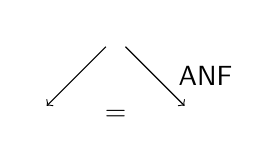
\begin{tikzpicture}
			[node distance=20mm, auto, transform shape]
			\node (m) at (0,0) {$\termone$};
			\node (n) at (-1,-1) {$\termtwo$};
			\node (l) at (1,-1) {$\termthree$};
			\node (eq) at (0,-1) {$=$};
			\draw (m) edge[->] node[left=5pt] {$\pslo$} (n);
			\draw (m) edge[->] node[right=5pt] {$\mathsf{ANF}$} (l);
			\end{tikzpicture}}}}
	\qquad
	\subfloat[]{{	
			\scalebox{0.9}{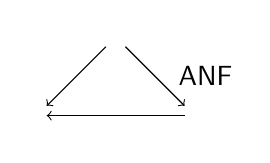
\begin{tikzpicture}
			[node distance=20mm, auto, transform shape]
			\node (m) at (0,0) {$\termone$};
			\node (n) at (-1,-1) {$\termtwo$};
			\node (l) at (1,-1) {$\termthree$};
			\draw (m) edge[->] node[left=5pt] {$\pslo$} (n);
			\draw (m) edge[->] node[right=5pt] {$\mathsf{ANF}$} (l);
			\draw (l) edge[->] node[below] {$\pslo$} (n);
			\end{tikzpicture}}}}\\
	\subfloat[]{{	
			\scalebox{0.9}{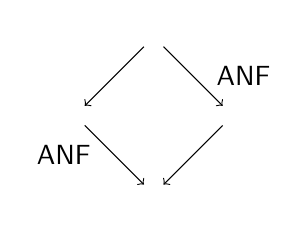
\begin{tikzpicture}
			[node distance=20mm, auto, transform shape]
			\node (m) at (0,0) {$\termone$};
			\node (n) at (-1,-1) {$\termtwo$};
			\node (l) at (1,-1) {$\termthree$};
			\node (p) at (0,-2) {$\termfour$};
			\draw (m) edge[->] node[left=5pt] {$\pslo$} (n);
			\draw (m) edge[->] node[right=5pt] {$\mathsf{ANF}$} (l);
			\draw (n) edge[->] node[left=5pt] {$\mathsf{ANF}$} (p);
			\draw (l) edge[->] node[right=5pt] {$\pslo$} (p);
			\end{tikzpicture}}}}
	\qquad
	\subfloat[]{{	
			\scalebox{0.9}{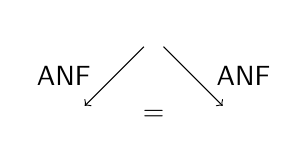
\begin{tikzpicture}
			[node distance=20mm, auto, transform shape]
			\node (m) at (0,0) {$\termone$};
			\node (n) at (-1,-1) {$\termtwo$};
			\node (l) at (1,-1) {$\termthree$};
			\node (eq) at (0,-1) {$=$};
			\draw (m) edge[->] node[left=5pt] {$\mathsf{ANF}$} (n);
			\draw (m) edge[->] node[right=5pt] {$\mathsf{ANF}$} (l);
			\end{tikzpicture}}}}
	\qquad
	\subfloat[]{{	
			\scalebox{0.9}{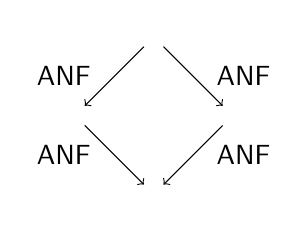
\begin{tikzpicture}
			[node distance=20mm, auto, transform shape]
			\node (m) at (0,0) {$\termone$};
			\node (n) at (-1,-1) {$\termtwo$};
			\node (l) at (1,-1) {$\termthree$};
			\node (p) at (0,-2) {$\termfour$};
			\draw (m) edge[->] node[left=5pt] {$\mathsf{ANF}$} (n);
			\draw (m) edge[->] node[right=5pt] {$\mathsf{ANF}$} (l);
			\draw (n) edge[->] node[left=5pt] {$\mathsf{ANF}$} (p);
			\draw (l) edge[->] node[right=5pt] {$\mathsf{ANF}$} (p);
			\end{tikzpicture}}}}
	\caption{The diagrams with the different cases of Lemma~\ref{lemma:LObase}.}
	\label{figure:diagramBase}
\end{figure}
\begin{lemma}\label{lemma:LOdiamond}
	If $\termone\redbetasteps{s}\termtwo$ and $\termone\redbetasteps{t}\termthree$ where $s,t\in\{\pslo,\mathsf{ANF}\}^*$ then there exist a term $\termfour$ such that $\termtwo\redbetasteps{u}\termfour$, $\termthree\redbetasteps{v}\termfour$, $\#_\pslo(s)+\#_\pslo(u)=\#_\pslo(t)+\#_\pslo(v)$, $|v|\leq |s|$ and $|u|\leq |t|$.
\end{lemma}
\begin{proof}
	By induction on $|s|+|t|$. The base case follows by Lemma~\ref{lemma:LObase}. Now suppose the statement true for $|s|+|t|\leq k-1$. We prove it for $|s|+|t|=k$. The idea is sketched in figure~\ref{figure:diagram}.  Let us consider the reductions $\termone\redbetardx{s_0}\termtwo'$ and $\termone\redbetardx{t_0}\termthree'$. By Lemma~\ref{lemma:LObase} there exist a term $\termfour'$ such that $\termtwo\redbetardx{u_0'}\termfour'$, $\termthree\redbetardx{v_0'}\termfour'$, $\#_\pslo(s_0)+\#_\pslo(u'_0)=\#_\pslo(t_0)+\#_\pslo(v_0')\leq 1$. By induction hypothesis since $\termtwo'\redbetasteps{s_{-1}}\termtwo$ and $\termtwo'\redbetasteps{u'_0}\termfour'$ there exists a term $\termfour''$ such that $\termtwo\redbetasteps{u''_0}\termfour''$, $\termfour'\redbetasteps{v''} \termfour''$, $\#_\pslo(s_{-1})+\#_\pslo(u''_0)=\#_\pslo(u'_0)+\#_\pslo(v'')$ and $|v''|\leq |s_{-1}|$. We can do the same with $\termthree'$ obtaining a term $\termfour'''$. Applying again the induction hypothesis to the reductions $\termfour'\redbetasteps{v''} \termfour''$ and $\termfour'\redbetasteps{u'''} \termfour'''$ we finally obtain a term $\termfour$ such that $\termfour''\redbetasteps{v''''} \termfour$, $\termfour'''\redbetasteps{u''''} \termfour$ and $\#_\pslo(v''')+\#_\pslo(u'''')=\#_\pslo(u''')+\#_\pslo(v'''')$. Summing up all the previous equalities and inequalities yields the result.
\end{proof}
\begin{figure}
	\centering
	\begin{tikzpicture}
	[node distance=20mm, auto, transform shape]
	\node (m) at (0,0) {$\termone$};
	\node (n') at (-1,-1) {$\termtwo'$};
	\node (l') at (1,-1) {$\termthree'$};
	\node (p') at (0,-2) {$\termfour'$};
	\node (n) at (-3,-3) {$\termtwo$};
	\node (p'') at (-2,-4) {$\termfour''$};
	\node (l) at (3,-3) {$\termthree$};
	\node (p''') at (2,-4) {$\termfour'''$};
	\node (p) at (0,-6) {$\termfour$};
	\draw (m) edge[->] node {} (n');
	\draw (m) edge[->] node {} (l');
	\draw (n') edge[->] node {} (p');
	\draw (l') edge[->] node {} (p');
	\draw (n') edge[->>] node {} (n);
	\draw (n) edge[->] node {} (p'');
	\draw (p') edge[->>] node {} (p'');
	\draw (l') edge[->>] node {} (l);
	\draw (l) edge[->] node {} (p''');
	\draw (p') edge[->] node {} (p''');
	\draw (p'') edge[->>] node {} (p);
	\draw (p''') edge[->>] node {} (p);
	\end{tikzpicture}
	\caption{The diagram representing the idea of the proof of Lemma~\ref{lemma:LOdiamond}.}
	\label{figure:diagram}
\end{figure}
\begin{corollary}\label{corollary:nfstring}
	If $\termone\in\Lambda_I$, $\termone\redbetasteps{\pslo\cdot s}\termtwo$, $\termone\redbetasteps{\mathsf{ANF}\cdot s}\termthree$, and $\termthree$ is in normal form, then $\termtwo$ is in normal form.
\end{corollary}
\begin{proof}
	By contraddiction suppose $\termtwo$ is not in normal form. By Lemma~\ref{lemma:LOdiamond} there exists a term $\termfour$ such that $\termtwo\redbetasteps{u}\termfour$, $\termthree\redbetasteps{v}\termfour$, and $\#_\pslo(\pslo\cdot s)+\#_\pslo(u)=\#_\pslo(\mathsf{ANF}\cdot s)+\#_\pslo(v)$. But since $\termthree$ is in normal form $|v|=0$. Thus after simple algebra the equality becomes $1+ \#_\pslo(s)+\#_\pslo(u)=\#_\pslo(s)$ i.e. $1+\#_\pslo(u)=0$, which is a contraddiction.
\end{proof}
\begin{proposition}
	For every probabilistic strategy $\mathsf{S}\in\psparamtwo{\varepsilon}$ if $\termone\in\Lambda_{\leq 1}$ then $\nsteps{\varepsilon}(\termone)$ is monotonically decreasing. 
\end{proposition}
\begin{proof}
	By induction on the maximum number of steps of $\termone$ to normal form.\\
	$\termone\redlo\termtwo$ with probability $\varepsilon$ and $\termone\redbetaanf\termthree$ with probability $1-\varepsilon$. Thus
	$$
	\nsteps{\varepsilon}(\termone) = \varepsilon\cdot\nsteps{\varepsilon}(\termtwo) + (1-\varepsilon)\cdot \nsteps{\varepsilon}(\termthree) + 1.
	$$
	Differentiating with respect to $\varepsilon$ we have
	$$
	\nsteps{\varepsilon}'(\termone) = \nsteps{\varepsilon}(\termtwo) + \varepsilon\cdot\nsteps{\varepsilon}'(\termtwo) -\nsteps{\varepsilon}(\termthree) + (1-\varepsilon)\cdot \nsteps{\varepsilon}'(\termthree).
	$$
	The thesis follows by Corollary~\ref{corollary:nfstring} and induction hypothesis.
\end{proof}